\documentclass[journal]{new-aiaa}
%DIF LATEXDIFF DIFFERENCE FILE
%DIF DEL /tmp/manuscript_before_round2.tex   Mon Nov 23 14:35:58 2026
%DIF ADD main.tex                            Mon Nov 23 14:30:28 2026
\usepackage[utf8]{inputenc}
\usepackage{graphicx,amsmath,longtable,tabularx,booktabs,placeins}
\renewcommand{\topfraction}{0.9}
\renewcommand{\bottomfraction}{0.8}
\renewcommand{\textfraction}{0.08}
\renewcommand{\floatpagefraction}{0.78}
\setcounter{topnumber}{3}
\setcounter{bottomnumber}{2}
\setcounter{totalnumber}{4}
\setlength\LTleft{0pt}
\newcommand{\CM}{C_M^A}
\newcommand{\degc}{^\circ}
% Primitive input keeps table rows expandable before booktabs rules.
\makeatletter
\newcommand{\tablerows}[1]{\@@input #1.tex }
\makeatother
\title{Pre-Stall Load Redistribution on Swept Tailplane Models with Full-Span Controls}
\author{Andrea Rausa\footnote{PhD, Department of Aerospace Science and Technology, Corresponding Author, andrea.rausa@polimi.it},
Alex Zanotti\footnote{Associate Professor, Department of Aerospace Science and Technology}, Giuseppe Gibertini\footnote{Associate Professor, Department of Aerospace Science and Technology}, Alberto Guardone\footnote{Full Professor, Department of Aerospace Science and Technology}, and Franco Auteri\footnote{Full Professor, Department of Aerospace Science and Technology}}
\affil{Politecnico di Milano, Department of Aerospace Science and Technology, Milano, Italy, 20154}
%DIF PREAMBLE EXTENSION ADDED BY LATEXDIFF
%DIF UNDERLINE PREAMBLE %DIF PREAMBLE
\RequirePackage[normalem]{ulem} %DIF PREAMBLE
\RequirePackage{color}\definecolor{RED}{rgb}{1,0,0}\definecolor{BLUE}{rgb}{0,0,1} %DIF PREAMBLE
\providecommand{\DIFadd}[1]{{\protect\color{blue}\uwave{#1}}} %DIF PREAMBLE
\providecommand{\DIFdel}[1]{{\protect\color{red}\sout{#1}}}                      %DIF PREAMBLE
%DIF SAFE PREAMBLE %DIF PREAMBLE
\providecommand{\DIFaddbegin}{} %DIF PREAMBLE
\providecommand{\DIFaddend}{} %DIF PREAMBLE
\providecommand{\DIFdelbegin}{} %DIF PREAMBLE
\providecommand{\DIFdelend}{} %DIF PREAMBLE
\providecommand{\DIFmodbegin}{} %DIF PREAMBLE
\providecommand{\DIFmodend}{} %DIF PREAMBLE
%DIF FLOATSAFE PREAMBLE %DIF PREAMBLE
\providecommand{\DIFaddFL}[1]{\DIFadd{#1}} %DIF PREAMBLE
\providecommand{\DIFdelFL}[1]{\DIFdel{#1}} %DIF PREAMBLE
\providecommand{\DIFaddbeginFL}{} %DIF PREAMBLE
\providecommand{\DIFaddendFL}{} %DIF PREAMBLE
\providecommand{\DIFdelbeginFL}{} %DIF PREAMBLE
\providecommand{\DIFdelendFL}{} %DIF PREAMBLE
\newcommand{\DIFscaledelfig}{0.5}
%DIF HIGHLIGHTGRAPHICS PREAMBLE %DIF PREAMBLE
\RequirePackage{settobox} %DIF PREAMBLE
\RequirePackage{letltxmacro} %DIF PREAMBLE
\newsavebox{\DIFdelgraphicsbox} %DIF PREAMBLE
\newlength{\DIFdelgraphicswidth} %DIF PREAMBLE
\newlength{\DIFdelgraphicsheight} %DIF PREAMBLE
% store original definition of \includegraphics %DIF PREAMBLE
\LetLtxMacro{\DIFOincludegraphics}{\includegraphics} %DIF PREAMBLE
\newcommand{\DIFaddincludegraphics}[2][]{{\color{blue}\fbox{\DIFOincludegraphics[#1]{#2}}}} %DIF PREAMBLE
\newcommand{\DIFdelincludegraphics}[2][]{% %DIF PREAMBLE
\sbox{\DIFdelgraphicsbox}{\DIFOincludegraphics[#1]{#2}}% %DIF PREAMBLE
\settoboxwidth{\DIFdelgraphicswidth}{\DIFdelgraphicsbox} %DIF PREAMBLE
\settoboxtotalheight{\DIFdelgraphicsheight}{\DIFdelgraphicsbox} %DIF PREAMBLE
\scalebox{\DIFscaledelfig}{% %DIF PREAMBLE
\parbox[b]{\DIFdelgraphicswidth}{\usebox{\DIFdelgraphicsbox}\\[-\baselineskip] \rule{\DIFdelgraphicswidth}{0em}}\llap{\resizebox{\DIFdelgraphicswidth}{\DIFdelgraphicsheight}{% %DIF PREAMBLE
\setlength{\unitlength}{\DIFdelgraphicswidth}% %DIF PREAMBLE
\begin{picture}(1,1)% %DIF PREAMBLE
\thicklines\linethickness{2pt} %DIF PREAMBLE
{\color[rgb]{1,0,0}\put(0,0){\framebox(1,1){}}}% %DIF PREAMBLE
{\color[rgb]{1,0,0}\put(0,0){\line( 1,1){1}}}% %DIF PREAMBLE
{\color[rgb]{1,0,0}\put(0,1){\line(1,-1){1}}}% %DIF PREAMBLE
\end{picture}% %DIF PREAMBLE
}\hspace*{3pt}}} %DIF PREAMBLE
} %DIF PREAMBLE
\LetLtxMacro{\DIFOaddbegin}{\DIFaddbegin} %DIF PREAMBLE
\LetLtxMacro{\DIFOaddend}{\DIFaddend} %DIF PREAMBLE
\LetLtxMacro{\DIFOdelbegin}{\DIFdelbegin} %DIF PREAMBLE
\LetLtxMacro{\DIFOdelend}{\DIFdelend} %DIF PREAMBLE
\DeclareRobustCommand{\DIFaddbegin}{\DIFOaddbegin \let\includegraphics\DIFaddincludegraphics} %DIF PREAMBLE
\DeclareRobustCommand{\DIFaddend}{\DIFOaddend \let\includegraphics\DIFOincludegraphics} %DIF PREAMBLE
\DeclareRobustCommand{\DIFdelbegin}{\DIFOdelbegin \let\includegraphics\DIFdelincludegraphics} %DIF PREAMBLE
\DeclareRobustCommand{\DIFdelend}{\DIFOaddend \let\includegraphics\DIFOincludegraphics} %DIF PREAMBLE
\LetLtxMacro{\DIFOaddbeginFL}{\DIFaddbeginFL} %DIF PREAMBLE
\LetLtxMacro{\DIFOaddendFL}{\DIFaddendFL} %DIF PREAMBLE
\LetLtxMacro{\DIFOdelbeginFL}{\DIFdelbeginFL} %DIF PREAMBLE
\LetLtxMacro{\DIFOdelendFL}{\DIFdelendFL} %DIF PREAMBLE
\DeclareRobustCommand{\DIFaddbeginFL}{\DIFOaddbeginFL \let\includegraphics\DIFaddincludegraphics} %DIF PREAMBLE
\DeclareRobustCommand{\DIFaddendFL}{\DIFOaddendFL \let\includegraphics\DIFOincludegraphics} %DIF PREAMBLE
\DeclareRobustCommand{\DIFdelbeginFL}{\DIFOdelbeginFL \let\includegraphics\DIFdelincludegraphics} %DIF PREAMBLE
\DeclareRobustCommand{\DIFdelendFL}{\DIFOaddendFL \let\includegraphics\DIFOincludegraphics} %DIF PREAMBLE
%DIF COLORLISTINGS PREAMBLE %DIF PREAMBLE
\RequirePackage{listings} %DIF PREAMBLE
\RequirePackage{color} %DIF PREAMBLE
\lstdefinelanguage{DIFcode}{ %DIF PREAMBLE
%DIF DIFCODE_UNDERLINE %DIF PREAMBLE
  moredelim=[il][\color{red}\sout]{\%DIF\ <\ }, %DIF PREAMBLE
  moredelim=[il][\color{blue}\uwave]{\%DIF\ >\ } %DIF PREAMBLE
} %DIF PREAMBLE
\lstdefinestyle{DIFverbatimstyle}{ %DIF PREAMBLE
	language=DIFcode, %DIF PREAMBLE
	basicstyle=\ttfamily, %DIF PREAMBLE
	columns=fullflexible, %DIF PREAMBLE
	keepspaces=true %DIF PREAMBLE
} %DIF PREAMBLE
\lstnewenvironment{DIFverbatim}{\lstset{style=DIFverbatimstyle}}{} %DIF PREAMBLE
\lstnewenvironment{DIFverbatim*}{\lstset{style=DIFverbatimstyle,showspaces=true}}{} %DIF PREAMBLE
%DIF END PREAMBLE EXTENSION ADDED BY LATEXDIFF

\begin{document}
\maketitle
\begin{abstract}
\label{anchor:abstract}
\DIFdelbegin \DIFdel{Local loading changes on a swept lifting surface with a deflected plain control can alter lift growth and pitching moment well before maximum lift . }\DIFdelend \DIFaddbegin \DIFadd{On swept wings with deflected trailing-edge controls, pitching moment can change while total lift continues to grow before stall. Integrated lift and moment coefficients reveal this behavior but do not identify how the loads on the fixed surface and control produce it. To investigate that relationship, }\DIFaddend MONNALISA wind-tunnel measurements \DIFdelbegin \DIFdel{and }\DIFdelend \DIFaddbegin \DIFadd{establish the aerodynamic response, while }\DIFaddend Reynolds-averaged Navier--Stokes \DIFdelbegin \DIFdel{calculations are used to examine how fixed-surface and full-span control loads combine in this response}\DIFdelend \DIFaddbegin \DIFadd{computations resolve the component and spatial loading}\DIFaddend . For the \DIFdelbegin \DIFdel{positive-sweep}\DIFdelend \DIFaddbegin \DIFadd{aft-swept reference model}\DIFaddend , \DIFdelbegin \DIFdel{zero-dihedral modelwith a 20$\degc$ control deflection, the computed }\DIFdelend \DIFaddbegin \DIFadd{the }\DIFaddend fixed surface continues gaining lift \DIFdelbegin \DIFdel{while both surface contributions fall below their preceding incidence trends. Across the tested fitting ranges, the fixed surface }\DIFdelend \DIFaddbegin \DIFadd{but }\DIFaddend accounts for about \DIFdelbegin \DIFdel{63\% }\DIFdelend \DIFaddbegin \DIFadd{two-thirds }\DIFaddend of the total \DIFdelbegin \DIFdel{lift departure; the }\DIFdelend \DIFaddbegin \DIFadd{shortfall relative to the preceding lift-growth trend. The }\DIFaddend control contributes more strongly to the \DIFdelbegin \DIFdel{moment }\DIFdelend \DIFaddbegin \DIFadd{pitching-moment }\DIFaddend departure about the \DIFdelbegin \DIFdel{fitted }\DIFdelend aerodynamic center. Pressure \DIFdelbegin \DIFdel{sections and regional integrations connect these different component contributions to }\DIFdelend \DIFaddbegin \DIFadd{distributions and spatially resolved load contributions show how }\DIFaddend stronger leading-edge suction \DIFdelbegin \DIFdel{, reduced hinge/aft loading, and longer outboard moment arms. Matched dihedral comparisons resolve incidence-dependent changes in lift growth and the force contributions to pitching moment}\DIFdelend \DIFaddbegin \DIFadd{coexists with reduced intermediate- and aft-chord loading, while the spanwise location of these changes governs their pitching-moment contributions. In the computed dihedral comparison, the higher-dihedral configuration has lower absolute lift but a larger increment over the selected pre-stall interval}\DIFaddend . The forward-swept planform \DIFdelbegin \DIFdel{gives weaker aft losses and a different spanwise distribution of moment contributions. The detailed interpretation concerns the computed flow fields and loads; agreement with measured integrated coefficients is partial. The combined force and moment analysis identifies loading changes that continuing total lift growth alone would conceal.
}%DIFDELCMD < 

%DIFDELCMD < %%%
\DIFdelend \DIFaddbegin \DIFadd{exhibits smaller aft-loading losses concentrated inboard. These results show how lift and pitching moment respond differently to spatial load redistribution.
}\DIFaddend \end{abstract}

\section*{Nomenclature}
\begin{longtable*}{@{}l@{\quad=\quad}l@{}}
$C_D,C_L$ & drag and lift coefficients \\
$C_{F,k}$ & body-force coefficient, $k=x,y,z$ \\
$C_M^A,C_M^O,C_M^{A_I}$ & moments about aerodynamic center, origin, or common configuration-I axis \\
$C_p,\ \mathbf C_f,C_{f,c}$ & pressure, vector skin-friction, and chordwise skin-friction coefficients \\
$D_{Q,j}$ & departure from the preceding coefficient trend \\
$F_k$ & body-force component, N \\
$\mathcal I_M$ & difference in moment increments between dihedral cases \\
$M_\infty$ & freestream Mach number \\
$Q$ & coefficient label, $L$ or $M$ \\
$Re_b,Re_{\bar c}$ & semispan and mean-chord Reynolds numbers \\
$S$ & \DIFdelbegin \DIFdel{undeformed semiplanform reference }\DIFdelend \DIFaddbegin \DIFadd{reference semiplanform }\DIFaddend area, m$^2$ \\
$T_\infty$ & freestream temperature, K \\
$U_\infty$ & freestream speed, m/s \\
$b$ & \DIFdelbegin \DIFdel{undeformed }\DIFdelend \DIFaddbegin \DIFadd{geometric }\DIFaddend semispan, m \\
$c,\ \bar c$ & local and mean aerodynamic chords, m \\
$f_{\mathrm{rev}}$ & upper control surface area fraction with reverse flow \\
$i,j,k$ & sample, surface-contribution, and force-component indices \\
$m_{Q,j}^{\mathrm{pre}}$ & preceding slope, per degree \\
$p,p_\infty$ & surface and freestream pressures, Pa \\
$q_\infty$ & freestream dynamic pressure, Pa \\
$s$ & \DIFdelbegin \DIFdel{undeformed span }\DIFdelend \DIFaddbegin \DIFadd{spanwise }\DIFaddend coordinate, m \\
$t$ & section thickness, m \\
$\mathbf t_c$ & downstream chordwise unit tangent \\
$u_i,w_i$ & supplied sample uncertainty magnitude and linear-combination weight \\
$u_{\mathrm{ind}},u_{\mathrm{L1}}$ & uncertainty sensitivities for coefficient departures \\
$x,y,z$ & downstream, spanwise, and upward body coordinates, m \\
$y^+$ & nondimensional wall distance \\
$x_A,x_O$ & aerodynamic-center and origin abscissae, m \\
$\alpha,\alpha_a,\alpha_b$ & incidence and interval endpoints, deg \\
$\Gamma,\delta$ & dihedral and control deflection, deg \\
$\Delta C_{Q,j}$ & actual coefficient increment \\
$\eta=s/b,\ \xi$ & span fraction and straightened local chord fraction \\
$\lambda,\Lambda$ & quarter-chord sweep (deg) and aspect ratio \\
$\rho_\infty$ & freestream density, kg/m$^3$ \\
$\tau,\boldsymbol\tau_w$ & taper ratio and wall-shear vector (Pa) \\
\end{longtable*}
% The unnumbered nomenclature must not consume a numbered-table entry.
\setcounter{table}{0}

\section{Introduction}\label{sec:intro}
A deflected trailing-edge control changes both \DIFdelbegin \DIFdel{the amount of lift generated by a lifting surface }\DIFdelend \DIFaddbegin \DIFadd{lift }\DIFaddend and the location \DIFdelbegin \DIFdel{at which }\DIFdelend \DIFaddbegin \DIFadd{where }\DIFaddend that load acts. \DIFdelbegin \DIFdel{Its response with incidence is therefore relevant to pitching moment as well as lift, even before the maximum-lift condition is reached. When local loading changes, total liftcan continue increasing while its growth slows and the pitching response changes more abruptly. Interpreting }\DIFdelend \DIFaddbegin \DIFadd{Consequently, the pitching moment can change abruptly even while total lift grows below stall. A local reduction in loading need not coincide with a reduction in integrated lift, because force contributions at different chordwise and spanwise positions combine. Explaining }\DIFaddend this behavior requires \DIFdelbegin \DIFdel{relating the integrated coefficients to the loads on the fixed and moving parts of the surface}\DIFdelend \DIFaddbegin \DIFadd{resolving fixed- and moving-surface loads rather than examining integrated coefficients alone}\DIFaddend .

\DIFdelbegin \DIFdel{Two-dimensional experiments on airfoils with plain flaps establish the starting point for this problem. }\DIFdelend \DIFaddbegin \DIFadd{Plain-flap experiments by }\DIFaddend Sears and Liddell~\cite{sears1942plain} \DIFdelbegin \DIFdel{measured lift, drag, pitching moment, and hinge moment for a 30\%-chord plain flap on an NACA 0015 airfoil, including sealed and unsealed hinge gaps. Separation }\DIFdelend \DIFaddbegin \DIFadd{documented }\DIFaddend reduced flap effectiveness \DIFaddbegin \DIFadd{associated with separation }\DIFaddend at large deflections\DIFdelbegin \DIFdel{, although additional deflection still increased lift within the tested range. Their comparison with a thinner symmetric section }\DIFdelend \DIFaddbegin \DIFadd{. They }\DIFaddend also showed that similar lift \DIFdelbegin \DIFdel{effectiveness could coexist with }\DIFdelend \DIFaddbegin \DIFadd{changes can accompany }\DIFaddend different hinge-moment behavior. \DIFdelbegin \DIFdel{Reduced flap effectiveness is thus established physics; neither separation nor a single integrated lift trend fully characterizes the loading response.
}%DIFDELCMD < 

%DIFDELCMD < %%%
\DIFdel{On a finite wing, flap-induced loading is also shaped by the spanwise flow and planform. Campbell, Blanks, and Leaver~\mbox{%DIFAUXCMD
\cite{campbell1956fullspan} }\hskip0pt%DIFAUXCMD
investigated rectangular wings of small aspect ratio }\DIFdelend \DIFaddbegin \DIFadd{On finite rectangular wings }\DIFaddend with full-span \DIFdelbegin \DIFdel{plain flapsof several chord fractions. Their force and pitching-moment measurements, compared with thin-wing theory and empirical thickness and boundary-layer allowances, related flap effectiveness and center of pressure to flap }\DIFdelend \DIFaddbegin \DIFadd{flaps, Campbell et al.~\mbox{%DIFAUXCMD
\cite{campbell1956fullspan} }\hskip0pt%DIFAUXCMD
related flap }\DIFaddend chord and aspect ratio \DIFdelbegin \DIFdel{. Those unswept, thinner, transition-tripped models differ from the present swept models, but they establish why the location of }\DIFdelend \DIFaddbegin \DIFadd{to lift and center of pressure. Together, these studies establish }\DIFaddend the \DIFdelbegin \DIFdel{additional load matters alongside its magnitude}\DIFdelend \DIFaddbegin \DIFadd{importance of both flap loading and the position of the resulting forces}\DIFaddend .



\DIFdelbegin \DIFdel{For }\DIFdelend \DIFaddbegin \DIFadd{On }\DIFaddend swept wings, \DIFdelbegin \DIFdel{Harper and Maki~\mbox{%DIFAUXCMD
\cite{harper1964sweptstall} }\hskip0pt%DIFAUXCMD
documented how }\DIFdelend spanwise changes in local lift \DIFdelbegin \DIFdel{response }\DIFdelend can produce pitching-moment nonlinearity \DIFdelbegin \DIFdel{below maximum lift. The first appearance }\DIFdelend \DIFaddbegin \DIFadd{before maximum lift~\mbox{%DIFAUXCMD
\cite{harper1964sweptstall}}\hskip0pt%DIFAUXCMD
. The onset }\DIFaddend of local stall need not coincide with the \DIFdelbegin \DIFdel{first integrated momentchange, because }\DIFdelend \DIFaddbegin \DIFadd{change in integrated moment: }\DIFaddend the force change and its moment arm vary along the span. \DIFdelbegin \DIFdel{Their broad stall review provides context for examining load redistribution , rather than an equivalent test of the present deflected-control configurations}\DIFdelend \DIFaddbegin \DIFadd{This motivates analyzing load redistribution instead of assigning a single global stall event}\DIFaddend .

Swept-flap experiments \DIFdelbegin \DIFdel{combining pressure, load, and flow-field measurements show that this spanwise organization extends to the flap flow itself. On a flapped NACA 0012 wing with adjustable sweep, }\DIFdelend \DIFaddbegin \DIFadd{reinforce this distinction. }\DIFaddend Tewes et al.~\cite{tewes2014sweepcontrol} found \DIFdelbegin \DIFdel{in the unactuated unswept configuration that the lift slope remained close to its thin-airfoil value although the flow over the deflected flap was separated , whereas the pitching moment increased as the separation location on the flap moved upstream. At 45$\degc$ sweep and zero incidence, the unactuated wing with a large flap deflection produced about half the lift of the unswept wing, and its pitching moment increased almost linearly with incidence instead of remaining constant. On a 30$\degc$ swept NACA 0015 }\DIFdelend \DIFaddbegin \DIFadd{that large deflection could produce separated flap flow with continued lift growth, while sweep altered the associated lift and pitching-moment response. Melton~\mbox{%DIFAUXCMD
\cite{melton2014sweptflap} }\hskip0pt%DIFAUXCMD
observed spanwise variation in separated flow on a swept }\DIFaddend wing with a 30\%-chord flap\DIFdelbegin \DIFdel{, Melton~\mbox{%DIFAUXCMD
\cite{melton2014sweptflap} }\hskip0pt%DIFAUXCMD
reported baseline pressure plateaus on the deflected flap, a large recirculation region near midspan with spanwise velocity directed toward the tip, and a smaller inboard recirculation region}\DIFdelend . These lower-Reynolds-number \DIFdelbegin \DIFdel{studies primarily address }\DIFdelend \DIFaddbegin \DIFadd{experiments primarily investigated }\DIFaddend active separation control and \DIFdelbegin \DIFdel{do not provide quantitative comparisons for the present models. Their unactuated results nevertheless show that flap separation can accompany continued lift growth while altering pitching moment, and that its extent varies along a swept span. They }\DIFdelend \DIFaddbegin \DIFadd{cannot validate the present configurations quantitatively. They establish context for the three-dimensional response but }\DIFaddend do not resolve \DIFdelbegin \DIFdel{how the fixed surface and flap separately contribute to those integrated changes}\DIFdelend \DIFaddbegin \DIFadd{the fixed- and control-surface contributions}\DIFaddend .

\DIFdelbegin \DIFdel{Nonlinear sectional data provide one route for representing these responses in reduced-order models. }\DIFdelend \DIFaddbegin \DIFadd{Reduced-order methods provide another perspective: }\DIFaddend Sivells and Neely~\cite{sivells1947liftingline} \DIFdelbegin \DIFdel{coupled such lift data to }\DIFdelend \DIFaddbegin \DIFadd{incorporated nonlinear sectional lift and moment data into }\DIFaddend lifting-line \DIFdelbegin \DIFdel{theory and also calculated wing pitching moment from sectional moment data . }\DIFdelend \DIFaddbegin \DIFadd{analysis, while }\DIFaddend Goitia and Llamas~\cite{goitia2019vlm} \DIFdelbegin \DIFdel{coupled a vortex-lattice formulation to }\DIFdelend \DIFaddbegin \DIFadd{combined }\DIFaddend viscous sectional data \DIFdelbegin \DIFdel{, with effective-sweep }\DIFdelend \DIFaddbegin \DIFadd{with vortex-lattice }\DIFaddend and finite-wing corrections\DIFdelbegin \DIFdel{, to predict nonlinear wing and tail lift. Consequently, a reduced-order model's ability to reproduce the response depends on how it represents sectional nonlinearities and changes in three-dimensional loading}\DIFdelend \DIFaddbegin \DIFadd{. Such formulations can predict nonlinear loading and pitching moment, while the present RANS solutions resolve the surface pressure and wall shear used to examine where those loads change}\DIFaddend .

The \DIFdelbegin \DIFdel{immediate basis for the present work is the MONNALISA database publication~\mbox{%DIFAUXCMD
\cite{rausa2026monnalisa} }\hskip0pt%DIFAUXCMD
. Sec.~IV and Fig.~11 already document the baseline }\DIFdelend \DIFaddbegin \DIFadd{MONNALISA database study~\mbox{%DIFAUXCMD
\cite{rausa2026monnalisa} }\hskip0pt%DIFAUXCMD
documented }\DIFaddend pre-stall lift nonlinearity, \DIFdelbegin \DIFdel{the expansion of }\DIFdelend reverse flow on the control, \DIFdelbegin \DIFdel{the }\DIFdelend associated pressure changes, and \DIFdelbegin \DIFdel{the continued growth of total lift . Its computations with the DUST mid-fidelity solver of Tugnoli et al.~\mbox{%DIFAUXCMD
\cite{tugnoli2021dust} }\hskip0pt%DIFAUXCMD
use sectional tables and corrections}\DIFdelend \DIFaddbegin \DIFadd{continued total lift growth. Its DUST computations~\mbox{%DIFAUXCMD
\cite{tugnoli2021dust} }\hskip0pt%DIFAUXCMD
used nonlinear sectional data}\DIFaddend , while the \DIFdelbegin \DIFdel{retained }\DIFdelend potential-based \DIFdelbegin \DIFdel{panel and vortex-lattice predictions are }\DIFdelend \DIFaddbegin \DIFadd{calculations were }\DIFaddend smoother. The present \DIFdelbegin \DIFdel{loading analysis builds on these established observations .
}%DIFDELCMD < 

%DIFDELCMD < %%%
\DIFdel{The remaining loading questionis how changes }\DIFdelend \DIFaddbegin \DIFadd{study builds on those observations but addresses a different question: how the loads }\DIFaddend on the fixed surface and control combine \DIFdelbegin \DIFdel{to produce the joint lift and moment response.
Continued }\DIFdelend \DIFaddbegin \DIFadd{into lift and pitching-moment changes.
}

\DIFadd{An actual increase of }\DIFaddend fixed-surface lift \DIFdelbegin \DIFdel{growth, for example, }\DIFdelend does not establish that \DIFdelbegin \DIFdel{this contribution follows its preceding trend. Comparing }\DIFdelend \DIFaddbegin \DIFadd{its growth follows the preceding incidence trend; similarly, a control lift loss alone does not establish its contribution to pitching moment. We compare }\DIFaddend actual increments with \DIFdelbegin \DIFdel{departures from that trend identifies which components supply the reduced total growth, while spatial pressure integrations show why the relative component contributions can differ for moment . This study develops that quantitative interpretation from the existing Reynolds-averaged Navier--Stokes (RANS) solutions, first assessing their integrated coefficients against the measured response and its supplied uncertainty. Changes in control deflection and geometry then test how broadly the reference loading pattern persists within the dataset}\DIFdelend \DIFaddbegin \DIFadd{preceding-incidence trends, examine chordwise and spanwise lift and moment contributions, and relate them to pressure and skin-friction distributions. Integrated WT--RANS comparisons first delimit the interpretation of computed surface loads. The two dihedral orientations and the opposite-sweep planform then reveal how load magnitudes and moment arms influence the response}\DIFaddend .

The \DIFdelbegin \DIFdel{test articles }\DIFdelend \DIFaddbegin \DIFadd{models }\DIFaddend are isolated tailplane-inspired wings with full-span, 30\%-chord plain controls\DIFdelbegin \DIFdel{; no fuselage, wing wake, or complete-aircraft trim condition is represented. Dihedral is varied on the same planform, while a forward-swept planform provides the opposite sweep direction. These comparisons define the scope of the analysis but }\DIFdelend \DIFaddbegin \DIFadd{, without fuselage or wing wake. The results }\DIFaddend do not establish behavior for partial-span controls \DIFdelbegin \DIFdel{, other flap chords, or intermediate dihedral angles}\DIFdelend \DIFaddbegin \DIFadd{or untested geometries}\DIFaddend .

\label{end:sec:intro}
\section{Methodology}\label{sec:methods}
\subsection{Models and wind-tunnel setup}\label{sec:setup}
Wind-tunnel (WT) measurements \DIFdelbegin \DIFdel{establish the }\DIFdelend \DIFaddbegin \DIFadd{provide }\DIFaddend integrated lift and \DIFdelbegin \DIFdel{pitching-moment response, while }\DIFdelend \DIFaddbegin \DIFadd{moment; }\DIFaddend RANS surface loads \DIFdelbegin \DIFdel{identify the contributionsof the fixed surface and control. To examine dihedral, we investigate the reference aft-swept planform (configuration I ) at }\DIFdelend \DIFaddbegin \DIFadd{resolve their component contributions. Configuration I is aft swept, with }\DIFaddend $\Gamma=0\degc$ and \DIFdelbegin \DIFdel{$\Gamma=45\degc$, with its in-plane geometry unchanged. A forward-swept planform (configuration II ) provides the opposite sweep direction and }\DIFdelend \DIFaddbegin \DIFadd{$45\degc$; configuration II is forward swept and has }\DIFaddend a different overall planform\DIFdelbegin \DIFdel{response. The tables use labels I and II}\DIFdelend .

Both \DIFdelbegin \DIFdel{models use a symmetric section of constant profile along the undeformed semispan $b=1.6$~m, }\DIFdelend \DIFaddbegin \DIFadd{wings use a constant symmetric section }\DIFaddend with thickness ratio $t/c=9\%$, \DIFdelbegin \DIFdel{where $c$ is the local chord. Each model has }\DIFdelend \DIFaddbegin \DIFadd{geometric semispan $b=1.6$~m, and }\DIFaddend a full-span plain control hinged at 70\% chord. \DIFdelbegin \DIFdel{The reference surface $S$ is the undeformed semiplanform area , and $\bar c$ denotes its }\DIFdelend \DIFaddbegin \DIFadd{Coefficients use the reference semiplanform area $S$ and }\DIFaddend mean aerodynamic chord \DIFdelbegin \DIFdel{(MAC)}\DIFdelend \DIFaddbegin \DIFadd{$\bar c$, independent of dihedral rotation}\DIFaddend . Table~\ref{tab:geometry} \DIFdelbegin \DIFdel{gives the geometric parameters and coefficient references. The }\DIFdelend \DIFaddbegin \DIFadd{lists the geometry: }\DIFaddend quarter-chord sweep \DIFdelbegin \DIFdel{is }\DIFdelend $\lambda=+30\degc$ for configuration I and \DIFdelbegin \DIFdel{$\lambda=-15\degc$ for configuration II; positive dihedral }\DIFdelend \DIFaddbegin \DIFadd{$-15\degc$ for II. Positive }\DIFaddend $\Gamma$ raises the tip\DIFdelbegin \DIFdel{. We define }\DIFdelend \DIFaddbegin \DIFadd{; }\DIFaddend aspect ratio for the \DIFdelbegin \DIFdel{corresponding full planform as }\DIFdelend \DIFaddbegin \DIFadd{full wing is }\DIFaddend $\Lambda=2b^2/S$\DIFdelbegin \DIFdel{, and $\tau$ as the tip-to-root chord ratio}\DIFdelend . Configuration II also differs in taper, aspect ratio, \DIFdelbegin \DIFdel{MAC, and chord-based Reynolds number}\DIFdelend \DIFaddbegin \DIFadd{area, and chord}\DIFaddend , so the \DIFdelbegin \DIFdel{sweep comparison is interpreted through the overall planform response }\DIFdelend \DIFaddbegin \DIFadd{response cannot be attributed to sweep alone}\DIFaddend .

\begin{table}[htbp]\centering
\caption{Model geometry and coefficient reference quantities.}\label{tab:geometry}
\begin{tabular}{lccc}\toprule
Property & I, $\Gamma=0\degc$ & I, $\Gamma=45\degc$ & II, $\Gamma=0\degc$ \\\midrule
$\lambda$ (deg) & 30 & 30 & $-15$ \\
$\Lambda$ & 5.0 & 5.0 & 5.2 \\
$\tau$ & 0.4 & 0.4 & 0.6 \\
$S$ (m$^2$) & 1.024 & 1.024 & 0.984604 \\
$\bar c$ (m) & 0.679184 & 0.679184 & 0.6282 \\
Root chord (m, rounded) & 0.914286 & 0.914286 & 0.76923 \\
$Re_{\bar c}$ & $2.335\times10^6$ & $2.335\times10^6$ & $2.159\times10^6$ \\
Numerical $x_A$ (m) & 0.642000 & 0.643532 & $-0.003618$ \\\bottomrule
\end{tabular}
\end{table}

\begin{figure}[htbp]\centering
\begin{minipage}[c]{.30\textwidth}\centering
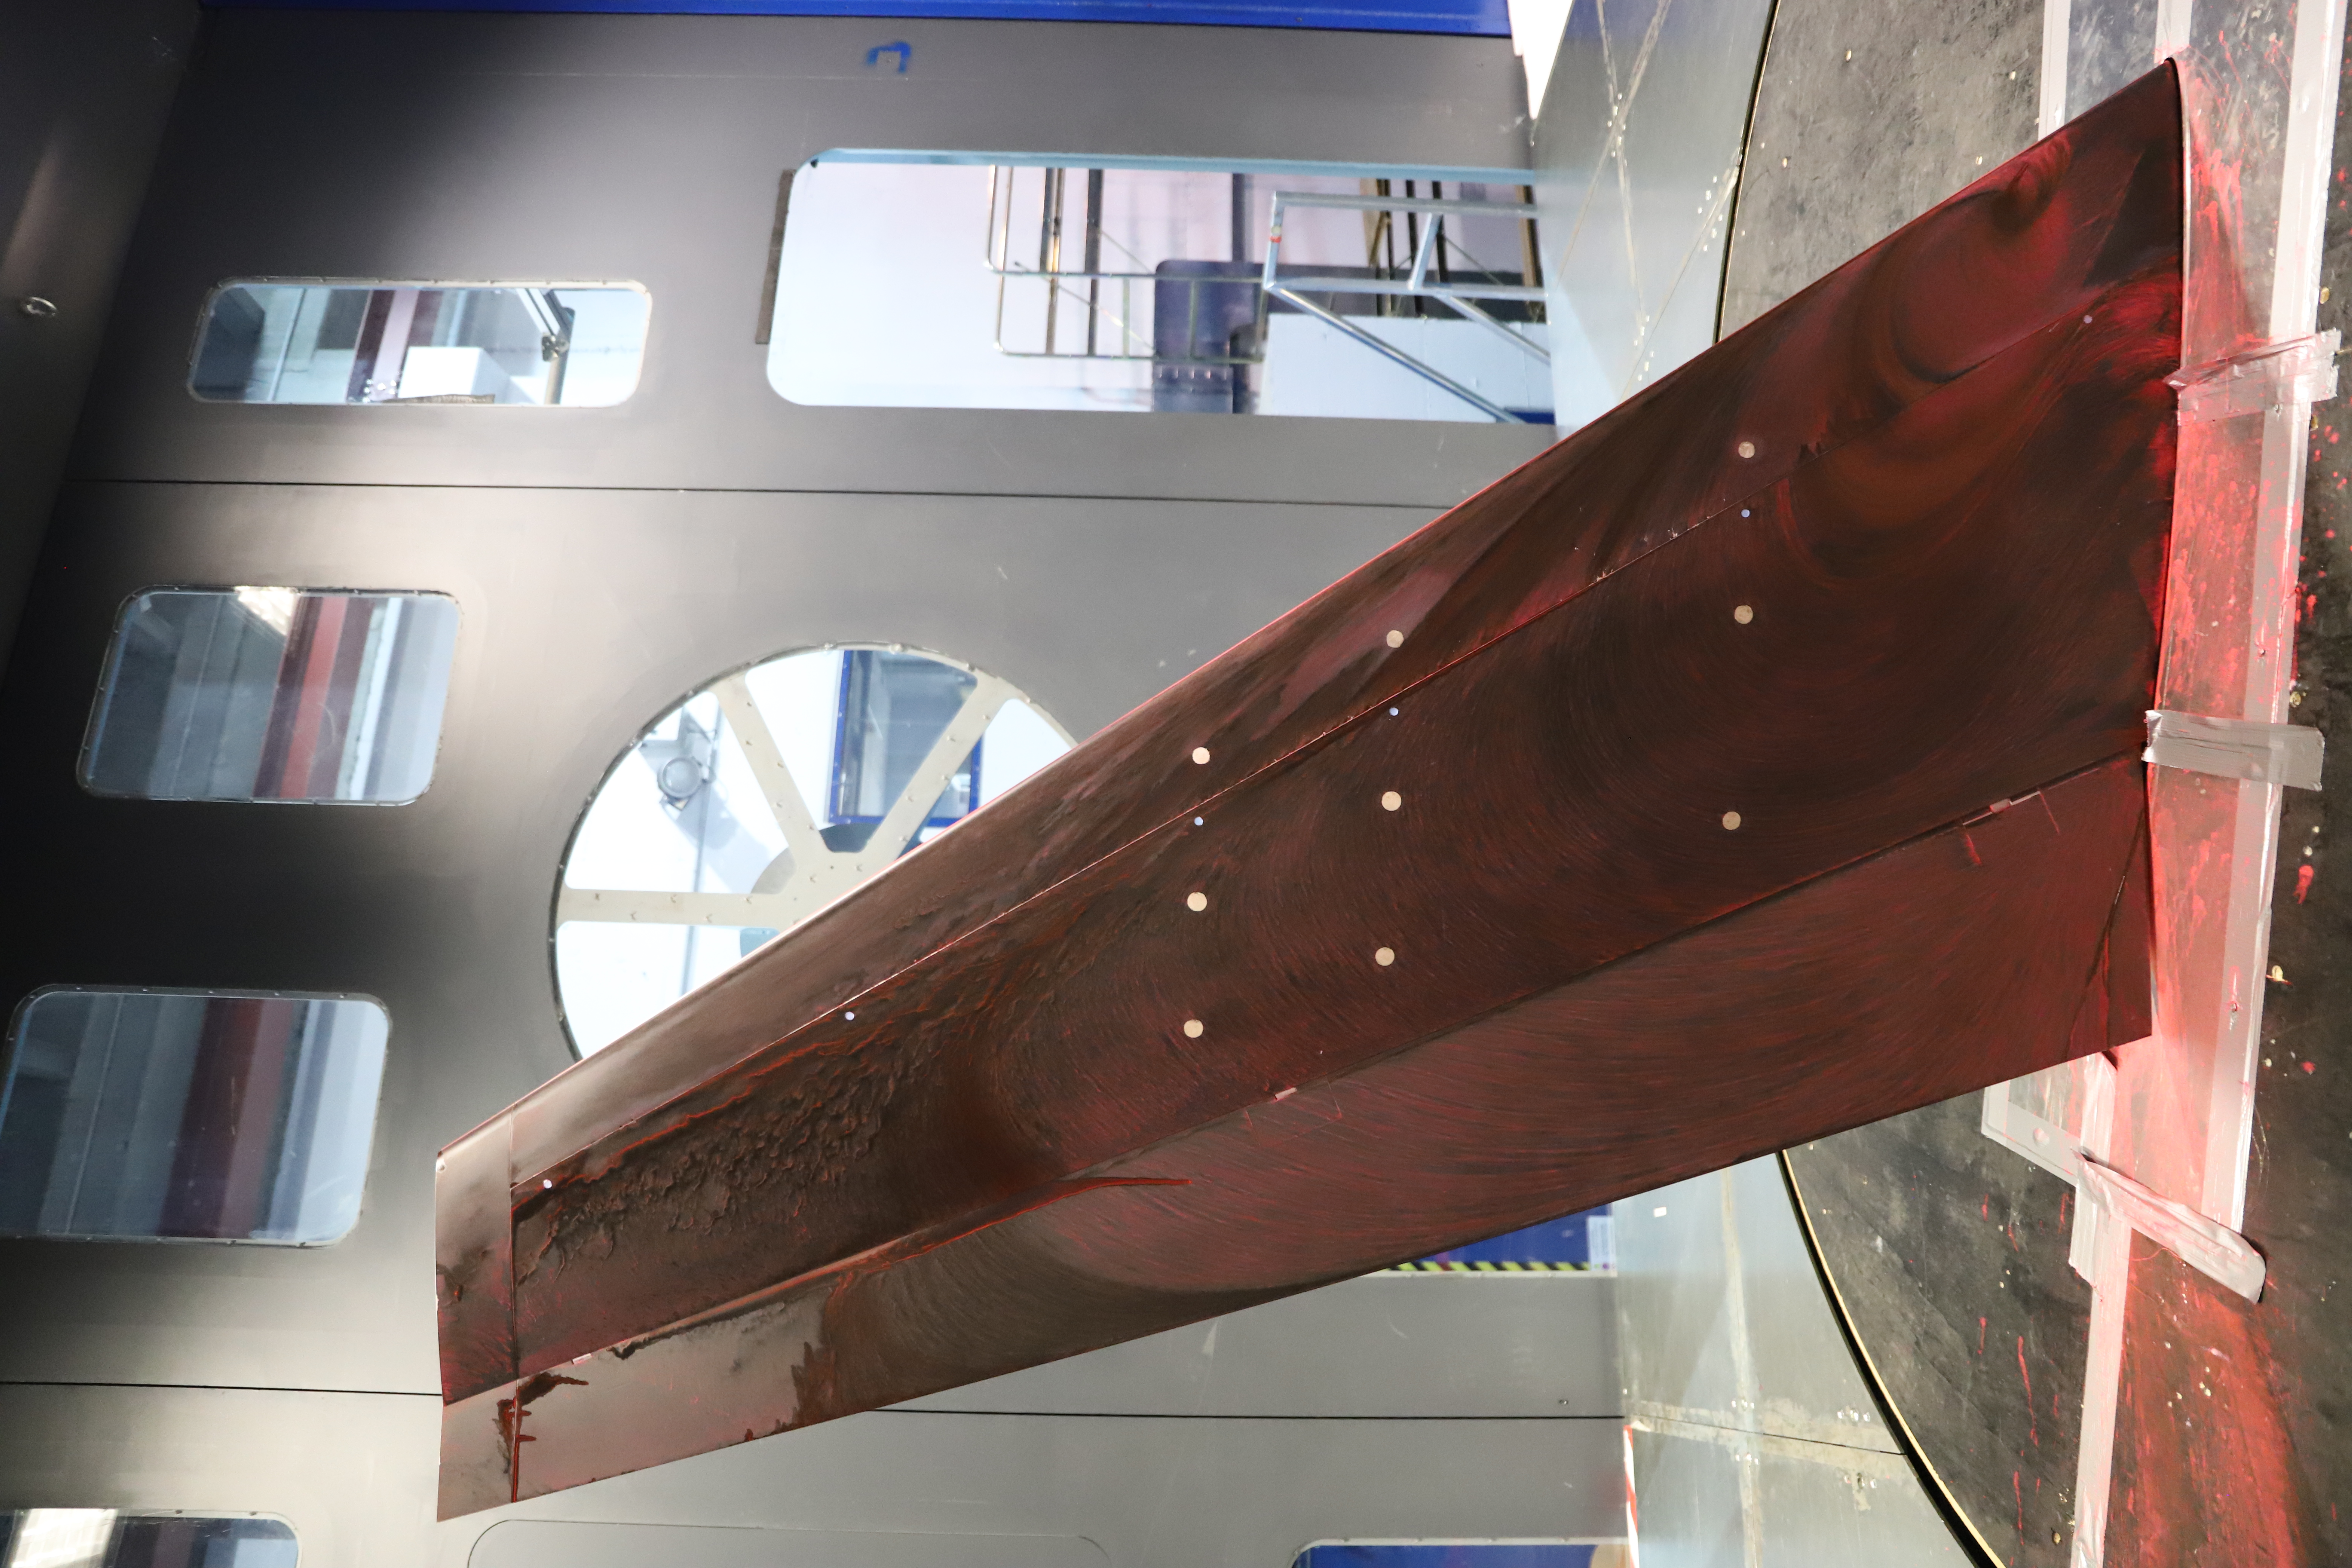
\includegraphics[angle=-90,origin=c,width=\linewidth]{figures_revision_installation.JPG}\\(a)
\end{minipage}\hfill
\begin{minipage}[c]{.65\textwidth}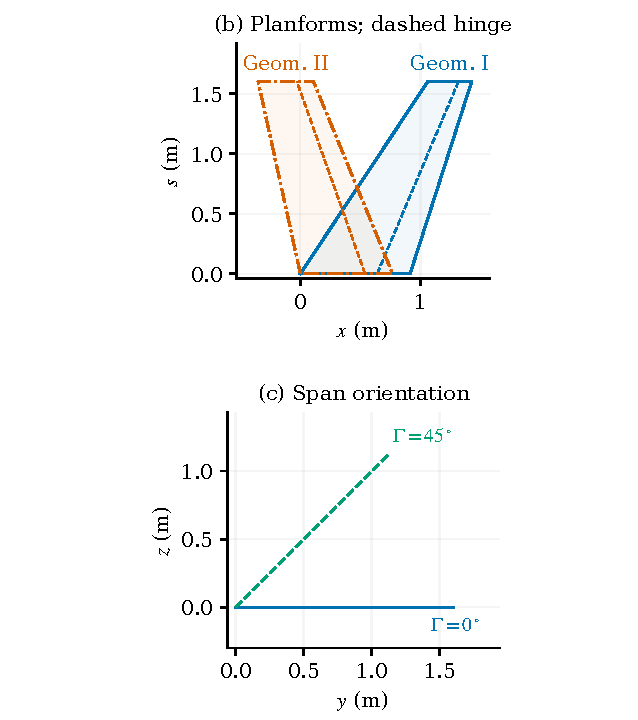
\includegraphics[width=\linewidth]{figures_revision_geometry.pdf}\end{minipage}
\caption{Wind-tunnel installation and geometry: (a) mounted semispan model; (b) reference and forward-swept planforms; (c) zero- and positive-dihedral arrangements.}\label{fig:setup}
\end{figure}

\DIFdelbegin \DIFdel{We obtained the measurements in the low-turbulence section of the }\DIFdelend \DIFaddbegin \DIFadd{Measurements were obtained in the }\DIFaddend Galleria del Vento del Politecnico di Milano\DIFdelbegin \DIFdel{(GVPM)}\DIFdelend , a closed-circuit \DIFdelbegin \DIFdel{facility. The test section is }\DIFdelend \DIFaddbegin \DIFadd{tunnel with a }\DIFaddend 4.00\DIFdelbegin \DIFdel{~m wide and }\DIFdelend \DIFaddbegin \DIFadd{-m-wide, }\DIFaddend 6.00\DIFdelbegin \DIFdel{~m long, with an original height of 3.84~m. For the present tests, installation of the }\DIFdelend \DIFaddbegin \DIFadd{-m-long test section. A raised }\DIFaddend false floor reduced \DIFdelbegin \DIFdel{the test-section height }\DIFdelend \DIFaddbegin \DIFadd{its height from 3.84 }\DIFaddend to 3.49~m; the \DIFdelbegin \DIFdel{undeformed model}\DIFdelend \DIFaddbegin \DIFadd{model's geometric }\DIFaddend semispan is 40\% of \DIFdelbegin \DIFdel{its width. A curved }\DIFdelend \DIFaddbegin \DIFadd{the tunnel width. An }\DIFaddend upstream inlet and gap beneath the \DIFdelbegin \DIFdel{false }\DIFdelend floor were designed to divert the incoming \DIFdelbegin \DIFdel{tunnel-floor boundary layerbelow the model installation. Boundary-layer development }\DIFdelend \DIFaddbegin \DIFadd{floor boundary layer. A new boundary layer developed }\DIFaddend over the raised floor and around the support\DIFdelbegin \DIFdel{remains distinct from a numerical symmetry boundary. The installation photograph in Fig. ~\ref{fig:setup} was taken }\DIFdelend \DIFaddbegin \DIFadd{, neither of which is represented by the numerical root symmetry condition. Figure~\ref{fig:setup} shows the installation }\DIFaddend at $\alpha=25\degc$, $\delta=20\degc$\DIFdelbegin \DIFdel{and shows the mounting , not }\DIFdelend \DIFaddbegin \DIFadd{; this photograph documents the mounting rather than }\DIFaddend the pre-stall flow\DIFdelbegin \DIFdel{conditions}\DIFdelend .

The database\DIFdelbegin \DIFdel{setup description~\mbox{%DIFAUXCMD
\cite{rausa2026monnalisa} }\hskip0pt%DIFAUXCMD
gives }\DIFdelend \DIFaddbegin \DIFadd{~\mbox{%DIFAUXCMD
\cite{rausa2026monnalisa} }\hskip0pt%DIFAUXCMD
reports }\DIFaddend freestream turbulence below 0.1\% \DIFdelbegin \DIFdel{, measured using a turbulence sphere and hot-wire anemometry. Outside }\DIFdelend \DIFaddbegin \DIFadd{and total-pressure variation outside }\DIFaddend the wall layers \DIFdelbegin \DIFdel{, the inlet total-pressure variation was }\DIFdelend within $\pm0.5\%$ of dynamic pressure over most of the section \DIFdelbegin \DIFdel{and within }\DIFdelend \DIFaddbegin \DIFadd{(}\DIFaddend $\pm1\%$ overall\DIFdelbegin \DIFdel{; outlet measurements confirmed similar uniformity. The reported }\DIFdelend \DIFaddbegin \DIFadd{), with a }\DIFaddend longitudinal static-pressure gradient \DIFdelbegin \DIFdel{is }\DIFdelend $\partial C_P/\partial x=-0.004$~m$^{-1}$. \DIFdelbegin \DIFdel{We acquired loads using a }\DIFdelend \DIFaddbegin \DIFadd{A }\DIFaddend RUAG 767 strain-gauge balance \DIFdelbegin \DIFdel{below the floor and an }\DIFdelend \DIFaddbegin \DIFadd{and }\DIFaddend HBM QuantumX system \DIFdelbegin \DIFdel{; the reduction includes the balance-to-wind transformation and database corrections}\DIFdelend \DIFaddbegin \DIFadd{supplied the forces and moments}\DIFaddend . The nominal \DIFdelbegin \DIFdel{freestream Mach number and temperature are }\DIFdelend \DIFaddbegin \DIFadd{operating point was }\DIFaddend $M_\infty=0.147$\DIFdelbegin \DIFdel{and }\DIFdelend \DIFaddbegin \DIFadd{, }\DIFaddend $T_\infty=300$~K, and \DIFaddbegin \DIFadd{span-based $Re_b=5.5\times10^6$. }\DIFaddend Table~\ref{tab:geometry} \DIFdelbegin \DIFdel{lists the MAC Reynolds numbers. The common database operating point is $Re_b=5.5\times10^6$; the MAC-based values are }\DIFdelend \DIFaddbegin \DIFadd{reports chord-based Reynolds numbers, obtained from }\DIFaddend $Re_{\bar c}=Re_b\bar c/b$.

\label{anchor:wt_uncertainty}\DIFdelbegin \DIFdel{Recorded incidences are $\alpha=-25,-24,-22,\ldots,22,24,25\degc$: the local }\DIFdelend \DIFaddbegin \DIFadd{Measured incidence extended from approximately $-25\degc$ to $25\degc$, with $2\degc$ spacing around the }\DIFaddend pre-stall \DIFdelbegin \DIFdel{spacing is $\Delta\alpha=2\degc$, with $\Delta\alpha=1\degc$ endpoint steps. The comparisons use }\DIFdelend \DIFaddbegin \DIFadd{changes and control deflections }\DIFaddend $\delta=0,10,20,30\degc$. \DIFdelbegin \DIFdel{Uncertainty bars are the supplied propagated measurement/reduction-chain }\DIFdelend \DIFaddbegin \DIFadd{The experimental bars are supplied propagated uncertainty }\DIFaddend magnitudes, including \DIFdelbegin \DIFdel{balance and transformation contributions. Each moment about the corresponding aerodynamic center retains its associated propagated uncertainty. The uncertainty sensitivities below use these supplied magnitudes }\DIFdelend \DIFaddbegin \DIFadd{the strain-gauge balance and balance-to-wind transformation, not statistical scatter from repeat runs. Moment uncertainties correspond to moments about the fitted aerodynamic centers. These magnitudes also underpin the departure sensitivity analysis in Sec.~\ref{sec:analysis}}\DIFaddend .

\label{end:sec:setup}
\subsection{Conventions and moment references}\label{sec:references}
Positive incidence \DIFdelbegin \DIFdel{$\alpha$ }\DIFdelend raises the leading edge\DIFdelbegin \DIFdel{relative to the freestream, and }\DIFdelend \DIFaddbegin \DIFadd{, }\DIFaddend positive control deflection \DIFdelbegin \DIFdel{$\delta$ }\DIFdelend moves the trailing edge downward\DIFdelbegin \DIFdel{relative to the fixed section. Lift is positive toward the upper surface and }\DIFdelend \DIFaddbegin \DIFadd{, and positive }\DIFaddend pitching moment is \DIFdelbegin \DIFdel{positive }\DIFdelend nose-up. \DIFdelbegin \DIFdel{The WT and numerical data are expressed in these common physical conventions. In body axes , }\DIFdelend \DIFaddbegin \DIFadd{Body axes are downstream (}\DIFaddend $x$\DIFdelbegin \DIFdel{is downstream , }\DIFdelend \DIFaddbegin \DIFadd{), spanwise (}\DIFaddend $y$\DIFdelbegin \DIFdel{is spanwise , and }\DIFdelend \DIFaddbegin \DIFadd{) and upward (}\DIFaddend $z$\DIFdelbegin \DIFdel{is upward. The axial force is the downstream body-axis component $F_x$, and the body-normal force is the upward component $F_z$. We define the latter in the common body frame, rather than normal to a panel tilted by dihedral. The body-force components $F_k$, with $k=x,y,z$, }\DIFdelend \DIFaddbegin \DIFadd{). Forces }\DIFaddend are normalized by \DIFdelbegin \DIFdel{the freestream dynamic pressure $q_\infty=\rho_\infty U_\infty^2/2$ and area $S$, where $\rho_\infty$ and $U_\infty$ are freestream density and speed. Lift and drag coefficients follow from }\DIFdelend \DIFaddbegin \DIFadd{$q_\infty S$; lift and drag follow from the body-axis components:
}\DIFaddend \begin{equation}
 C_L=C_{F,z}\cos\alpha-C_{F,x}\sin\alpha,\qquad
 C_D=C_{F,z}\sin\alpha+C_{F,x}\cos\alpha,\qquad
 C_{F,k}=F_k/(q_\infty S).
\label{eq:force}
\end{equation}
Pitching moment is normalized by $q_\infty S\bar c$. Body coordinates are expressed relative to the root leading edge.

\label{anchor:fitted_reference}\DIFdelbegin \DIFdel{Both experimental and numerical moments are referred to aerodynamic centers determined from the }\DIFdelend \DIFaddbegin \DIFadd{Experimental and numerical aerodynamic centers are fitted separately from }\DIFaddend zero-deflection \DIFdelbegin \DIFdel{loading characteristics. Linear fits to moment and body-normal force }\DIFdelend \DIFaddbegin \DIFadd{moment and body-normal-force trends }\DIFaddend over $|\alpha|\leq10\degc$ \DIFdelbegin \DIFdel{define the positions, which remain fixed when control deflection varies}\DIFdelend \DIFaddbegin \DIFadd{and then fixed as control deflection changes}\DIFaddend ~\cite{rausa2026monnalisa}. \DIFdelbegin \DIFdel{The experimental fits use the supplied uncertainty weights; the numerical fits use the retained zero-deflection linear trends. }\DIFdelend For configuration I, \DIFdelbegin \DIFdel{the WTand }\DIFdelend \DIFaddbegin \DIFadd{WT/}\DIFaddend RANS positions are \DIFdelbegin \DIFdel{0.6430 and 0.6420}\DIFdelend \DIFaddbegin \DIFadd{$0.6430/0.6420$}\DIFaddend ~m at zero dihedral \DIFdelbegin \DIFdel{, and 0.6455 and 0.6435}\DIFdelend \DIFaddbegin \DIFadd{and $0.6455/0.6435$}\DIFaddend ~m at \DIFdelbegin \DIFdel{$\Gamma=45\degc$: separations of about 1.0 and 2.0}\DIFdelend \DIFaddbegin \DIFadd{$45\degc$, differences of about 1 and 2}\DIFaddend ~mm. For \DIFdelbegin \DIFdel{configuration II, they are $-0.0492$ and $-0.00362$}\DIFdelend \DIFaddbegin \DIFadd{II, the positions are $-0.0492/-0.00362$}\DIFaddend ~m, \DIFdelbegin \DIFdel{separated }\DIFdelend \DIFaddbegin \DIFadd{differing }\DIFaddend by 45.6~mm. \DIFdelbegin \DIFdel{The comparison coefficient $\CM$ therefore uses the same reference construction , with each dataset's fitted position; it is not an imposed quarter-MAC moment }\DIFdelend \DIFaddbegin \DIFadd{Thus matching the reference construction does not impose identical moment axes on WT and RANS; the common-axis dihedral diagnostic below explicitly uses one physical reference}\DIFaddend .

The original numerical reference is $O=(0.228571,0,0)$~m, the root quarter-chord of Geom.~I. For a numerical pole transported from abscissa $x_0$ to $x_1$,
\begin{equation}
 C_M(x_1)=C_M(x_0)+\frac{x_1-x_0}{\bar c}C_{F,z}.
\label{eq:transport}
\end{equation}
Table~\ref{tab:geometry} lists the fitted abscissae. Matched dihedral diagnostics use the identical numerical axis $A_I=(0.642000,0,0)$~m in both configurations, denoted $C_M^{A_I}$. Geom.~II uses its own MAC once for every moment contribution; all coefficients use the fixed areas in Table~\ref{tab:geometry}.

\label{end:sec:references}
\subsection{Numerical setup}\label{sec:numerics}
\DIFdelbegin \DIFdel{The }\DIFdelend SU2~\cite{palacios2013stanford} \DIFdelbegin \DIFdel{calculations solve }\DIFdelend \DIFaddbegin \DIFadd{solves }\DIFaddend compressible ideal-gas RANS with Sutherland viscosity, \DIFdelbegin \DIFdel{the }\DIFdelend Spalart--Allmaras \DIFdelbegin \DIFdel{(SA) turbulencemodel}\DIFdelend \DIFaddbegin \DIFadd{turbulence}\DIFaddend ~\cite{spalart1992sa}, and the Bas--Cakmakcioglu \DIFdelbegin \DIFdel{(BCM) algebraic transition treatment}\DIFdelend \DIFaddbegin \DIFadd{transition model}\DIFaddend ~\cite{cakmakcioglu2020bcm}. \DIFdelbegin \DIFdel{The finite-volume mean-flow discretization uses }\DIFdelend \DIFaddbegin \DIFadd{Vertex-centered }\DIFaddend median-dual \DIFdelbegin \DIFdel{vertex cells , }\DIFdelend \DIFaddbegin \DIFadd{cells use }\DIFaddend Roe fluxes, second-order \DIFdelbegin \DIFdel{monotonic upstream-centered schemes for conservation laws (MUSCL ) }\DIFdelend \DIFaddbegin \DIFadd{MUSCL }\DIFaddend reconstruction~\cite{van1979towards}, Green--Gauss gradients \DIFdelbegin \DIFdel{, }\DIFdelend and a Venkatakrishnan limiter~\cite{venkatakrishnan1993accuracy} \DIFdelbegin \DIFdel{with }\DIFdelend \DIFaddbegin \DIFadd{(}\DIFaddend coefficient 0.05\DIFdelbegin \DIFdel{. SA }\DIFdelend \DIFaddbegin \DIFadd{); turbulence }\DIFaddend convection uses first-order \DIFdelbegin \DIFdel{scalar }\DIFdelend upwinding.

\label{anchor:wall_model}The \DIFdelbegin \DIFdel{model surfaces have }\DIFdelend \DIFaddbegin \DIFadd{wing has }\DIFaddend no-slip, adiabatic \DIFdelbegin \DIFdel{boundaries, with freestream conditions at the far field and symmetry at the root . The symmetry plane omits the physical support and boundary-layer development over the raised-floor arrangement. Steady solutions use implicit Euler}\DIFdelend \DIFaddbegin \DIFadd{walls, freestream far-field and root symmetry boundaries. Steady }\DIFaddend pseudo-time \DIFdelbegin \DIFdel{advancement and flexible generalized minimal residual (FGMRES) linear solves, with an adaptive Courant--Friedrichs--Lewy (CFL) number. The production stopping criterion monitors liftand drag over 100 entries with a Cauchy tolerance of }\DIFdelend \DIFaddbegin \DIFadd{iteration uses implicit Euler, FGMRES and adaptive CFL. The lift/drag Cauchy stopping tolerance is }\DIFaddend approximately $3\times10^{-6}$ \DIFaddbegin \DIFadd{over 100 entries}\DIFaddend .

\DIFdelbegin \DIFdel{The surface grid resolves }\DIFdelend \DIFaddbegin \DIFadd{Hex-dominant, octree-based meshes~\mbox{%DIFAUXCMD
\cite{rausa2026monnalisa} }\hskip0pt%DIFAUXCMD
resolve }\DIFaddend the leading edge, hinge junction, \DIFdelbegin \DIFdel{and }\DIFdelend trailing edge, \DIFdelbegin \DIFdel{where curvature and pressure changes require additional resolution. Wall-normal boundary-layer extrusion uses a }\DIFdelend \DIFaddbegin \DIFadd{and incidence-dependent wake. Boundary-layer extrusion has }\DIFaddend nominal first-cell height \DIFdelbegin \DIFdel{of about }\DIFdelend $2\times10^{-6}$~m and growth ratio 1.15\DIFdelbegin \DIFdel{, while volume refinement follows the wake at each incidence. The volume mesh is hex-dominant and octree-based~\mbox{%DIFAUXCMD
\cite{rausa2026monnalisa}}\hskip0pt%DIFAUXCMD
. Representative solutions have median nondimensional wall distance }\DIFdelend \DIFaddbegin \DIFadd{. Representative median wall distance is }\DIFaddend $y^+=0.19$--0.26, with \DIFdelbegin \DIFdel{local maxima about }\DIFdelend \DIFaddbegin \DIFadd{maxima }\DIFaddend 1.1--1.3.
\DIFdelbegin \DIFdel{A reference grid contains approximately 9.44 million points and 18.92 million volume elements.
}%DIFDELCMD < 

%DIFDELCMD < %%%
\DIFdel{The existing grid-refinement assessment uses four levels---coarse, nominal, fine, and very fine---for configuration I at }\DIFdelend \DIFaddbegin 

\DIFadd{A four-level grid study on configuration I used }\DIFaddend $\delta=35\degc$, $\Gamma=0,45\degc$ \DIFdelbegin \DIFdel{, }\DIFdelend and $\alpha=0,18\degc$ \DIFdelbegin \DIFdel{. }\DIFdelend \DIFaddbegin \DIFadd{(}\DIFaddend Table~\ref{tab:mesh}\DIFdelbegin \DIFdel{gives the point and element ranges.Figure~\ref{fig:mesh}compares lift, drag, and pitching moment against the actual grid-point count on a logarithmic scale; open squares identify the nominal level, and lines connect the retained levels. Moments are about the numerical origin $O$, using the configuration-I area and MAC.
}%DIFDELCMD < 

%DIFDELCMD < %%%
\DIFdel{The nominal level balances spatial resolution with the demands of the extensive MONNALISA campaign across geometries, incidences, and control deflections. Its approximately }\DIFdelend \DIFaddbegin \DIFadd{, Fig.~\ref{fig:mesh}). Nominal meshes had }\DIFaddend 9.7--12.7 million points \DIFdelbegin \DIFdel{compare with }\DIFdelend \DIFaddbegin \DIFadd{versus }\DIFaddend 50.1--65.9 million on the finest level. \DIFaddbegin \DIFadd{Moments in Fig.~\ref{fig:mesh} use the original numerical pole.
}

\DIFaddend Nominal-to-finest differences \DIFdelbegin \DIFdel{are }\DIFdelend \DIFaddbegin \DIFadd{were }\DIFaddend 1.20--2.14\% \DIFdelbegin \DIFdel{for }\DIFdelend \DIFaddbegin \DIFadd{in }\DIFaddend lift and 1.13--2.49\% \DIFdelbegin \DIFdel{for }\DIFdelend \DIFaddbegin \DIFadd{in }\DIFaddend drag. At \DIFdelbegin \DIFdel{zero dihedral and }\DIFdelend \DIFaddbegin \DIFadd{$\Gamma=0\degc$, }\DIFaddend $\alpha=18\degc$, $C_M^O$ \DIFdelbegin \DIFdel{changes from approximately }\DIFdelend \DIFaddbegin \DIFadd{changed from }\DIFaddend $-0.813$ to $-0.827$\DIFdelbegin \DIFdel{, an absolute difference of 0.0134; the $\Gamma=45\degc$ moment sequence is }\DIFdelend \DIFaddbegin \DIFadd{; the $45\degc$ moment sequence was }\DIFaddend nonmonotonic. The \DIFdelbegin \DIFdel{assessment supports the nominal grid as a practical production compromise while showing finite, condition-dependent integrated-load sensitivity. It provides }\DIFdelend \DIFaddbegin \DIFadd{nominal mesh reduced campaign cost but gives }\DIFaddend no discretization-error bound for local component loads.
\DIFdelbegin \DIFdel{The comparison with measurements in Sec.~\ref{sec:response} separately assesses reproduction of the principal pre-stall aerodynamic trends.
}\DIFdelend 

\begin{table}[htbp]\centering
\caption{Point and volume-element ranges, in millions, for the four-level refinement assessment.}\label{tab:mesh}
\begin{tabular}{lrr}\toprule
Refinement & Points & Volume elements \\\midrule
Coarse & 4.79--5.29 & 9.51--10.90 \\
Nominal & 9.67--12.74 & 19.06--24.07 \\
Fine & 22.33--26.56 & 39.93--45.70 \\
Very fine & 50.11--65.89 & 87.35--109.98 \\
\bottomrule\end{tabular}\end{table}

\begin{figure}[htbp]\centering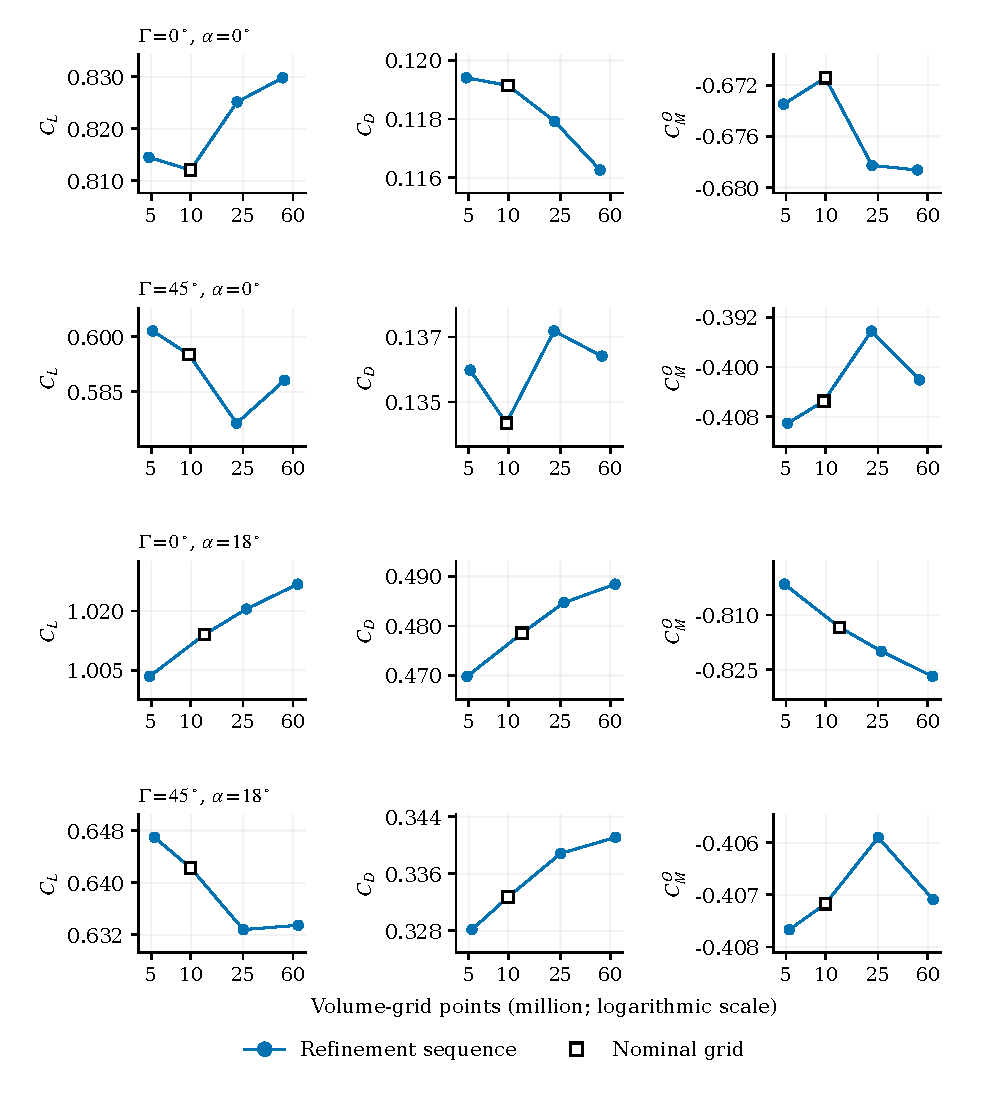
\includegraphics[width=\textwidth]{figures_revision_mesh_refinement.pdf}
\caption{Grid-refinement trends of lift, drag, and pitching moment for configuration I at $\delta=35\degc$, two incidences, and two dihedral settings.}\label{fig:mesh}\end{figure}

\label{end:sec:numerics}
\subsection{Load decomposition and trend departures}\label{sec:analysis}
\DIFdelbegin \DIFdel{A surface can gain lift and still contribute to a reduction in total lift growth. To distinguish these effects, the actual increment is the measured or computed change in the coefficient between two incidences. The expected increment is obtained by linearly extrapolating the }\DIFdelend \DIFaddbegin \DIFadd{An actual coefficient increment is its change over a sampled incidence interval. Its departure subtracts the increment predicted by continuing an }\DIFaddend empirically fitted preceding slope over the same interval. \DIFdelbegin \DIFdel{Their difference, actual minus expected, is the departure. For the fixed surface of configuration I at zero dihedral and }\DIFdelend \DIFaddbegin \DIFadd{At }\DIFaddend $\delta=20\degc$, \DIFdelbegin \DIFdel{the actual increase over }\DIFdelend $\alpha=0\to2\degc$\DIFdelbegin \DIFdel{is $+0.0593$, while continuation of the preceding trend predicts }\DIFdelend \DIFaddbegin \DIFadd{, for example, fixed-surface lift increases by $+0.0593$ rather than the predicted }\DIFaddend $+0.1285$\DIFdelbegin \DIFdel{. The }\DIFdelend \DIFaddbegin \DIFadd{: its }\DIFaddend departure is $-0.0692$\DIFdelbegin \DIFdel{: the fixed surface still gains lift, but gains 0.0692 less than predicted by that trend. This is a reduction in growth , not an actual lift loss }\DIFdelend \DIFaddbegin \DIFadd{. A negative departure therefore means reduced growth relative to the chosen reference, not necessarily an actual loss of lift}\DIFaddend .

\DIFdelbegin \DIFdel{The analysis resolves these changes into additive surface loads . Solver surface groups define the fixed surface (upper/lower fixedpanels), the control (upper/lower control panels, hinge junction }\DIFdelend \DIFaddbegin \DIFadd{We integrate pressure and viscous loads over fixed}\DIFaddend , \DIFaddbegin \DIFadd{control and tip surfaces using consistent reference quantities. The control includes the hinge junction }\DIFaddend and blunt trailing edge\DIFdelbegin \DIFdel{), and tip . Pressure and viscous contributions are retained on both physical sides with the same global $S$ and $\bar c$. Tip }\DIFdelend \DIFaddbegin \DIFadd{; tip }\DIFaddend loads remain in \DIFdelbegin \DIFdel{every total and closure check. All displayed coefficientsuse their actual magnitude}\DIFdelend \DIFaddbegin \DIFadd{total coefficients}\DIFaddend .

For \DIFdelbegin \DIFdel{coefficient label $Q=L$ or $M$ and surface contribution $j$ (fixed, control, tip, or total)}\DIFdelend \DIFaddbegin \DIFadd{lift or moment coefficient $Q$}\DIFaddend , the actual increment \DIFdelbegin \DIFdel{is the change between sampled incidences $\alpha_a$ and $\alpha_b$. Its departure subtracts the change predicted by continuing the preceding slope $m_{Q,j}^{\mathrm{pre}}$, measured per degree,
}\DIFdelend \DIFaddbegin \DIFadd{and departure of component $j$ are
}\DIFaddend \begin{equation}
 \Delta C_{Q,j}=C_{Q,j}(\alpha_b)-C_{Q,j}(\alpha_a),\qquad
 D_{Q,j}=\Delta C_{Q,j}-m_{Q,j}^{\mathrm{pre}}(\alpha_b-\alpha_a).
\label{eq:departure}
\end{equation}
\DIFdelbegin \DIFdel{The }\DIFdelend \DIFaddbegin \DIFadd{Each }\DIFaddend preceding slope is an unweighted \DIFdelbegin \DIFdel{linear }\DIFdelend least-squares fit \DIFdelbegin \DIFdel{to the specified preceding incidence samples. Using identical samples and weights for every component and the total preserves additivityfor both increments and departures. The primary preceding-incidence range }\DIFdelend \DIFaddbegin \DIFadd{using identical incidence samples }\DIFaddend for \DIFaddbegin \DIFadd{all load components, preserving additivity. For }\DIFaddend $\delta=20\degc$ \DIFaddbegin \DIFadd{the primary preceding range }\DIFaddend is $\alpha\in\{-6,-4,-2\}\degc$; \DIFdelbegin \DIFdel{the early reference }\DIFdelend \DIFaddbegin \DIFadd{for the early }\DIFaddend $\delta=30\degc$ \DIFdelbegin \DIFdel{numerical baseline is $\alpha\in\{-16,-14,-12\}\degc$. These are empirical references, with no assumption that the preceding flow is attached . Neighboring preceding-incidence fitting ranges test this reference dependence, with the same surface solutions. Where the preceding sequence is curved, signed finite differences describe the response without imposing a unique event amplitude}\DIFdelend \DIFaddbegin \DIFadd{feature it is $\{-16,-14,-12\}\degc$. These empirical slopes are not assumed to represent attached flow. Neighboring fitting windows quantify reference sensitivity, while finite differences remain meaningful when the preceding trend is curved}\DIFaddend .

\DIFdelbegin \DIFdel{We evaluate the uncertainty sensitivity of each measured lift or moment departure by propagating the supplied coefficient uncertainties through its defining linear combination. Equation~\ref{eq:departure} is written as $D=\sum_i w_iC_i$, where $i$ indexes the measured samples, $w_i$ is the combined coefficient weight, and $u_i$ is its supplied propagated uncertainty magnitude. The independence-based sensitivity $u_{\mathrm{ind}}$ and absolute-weight sensitivity $u_{\mathrm{L1}}$ are
}\DIFdelend \DIFaddbegin \DIFadd{Propagating the supplied measured-coefficient uncertainties through $D=\sum_i w_i C_i$ gives
}\DIFaddend \begin{equation}
 u_{\mathrm{ind}}=\left[\sum_i(w_i u_i)^2\right]^{1/2},\qquad
 u_{\mathrm{L1}}=\sum_i|w_i|u_i.
\label{eq:uncertainty}
\end{equation}
The first \DIFdelbegin \DIFdel{is conditional on independence; the second bounds a perturbation when each sample varies within }\DIFdelend \DIFaddbegin \DIFadd{assumes independent errors. The second bounds the combined perturbation if each sample error is bounded by }\DIFaddend its supplied magnitude\DIFdelbegin \DIFdel{. Coverage and between-incidence covariance are undocumented, so these quantify sensitivity to the supplied uncertainties rather than }\DIFdelend \DIFaddbegin \DIFadd{; unknown inter-incidence covariance and coverage prevent interpreting these sensitivities as }\DIFaddend confidence intervals.

\DIFdelbegin \DIFdel{To locate the changes identified by the component load decomposition, we integrate pressure }\DIFdelend \DIFaddbegin \DIFadd{Pressure }\DIFaddend and wall-shear forces \DIFaddbegin \DIFadd{are integrated on the triangulated surface }\DIFaddend over chordwise and spanwise regions. The pressure coefficient is $C_p=(p-p_\infty)/q_\infty$ \DIFdelbegin \DIFdel{, and the skin-friction vector is }\DIFdelend \DIFaddbegin \DIFadd{and wall-shear coefficient }\DIFaddend $\mathbf C_f=\boldsymbol\tau_w/q_\infty$\DIFdelbegin \DIFdel{, where $p_\infty$ is freestream pressure and $\boldsymbol\tau_w$ is wall shear. Linear surface tractions and their moments are integrated over the triangulated surface, with
}\begin{displaymath}
 \DIFdel{C_M(x_A)=\frac{1}{q_\infty S\bar c}
 \int\big[z\,dF_x-(x-x_A)dF_z\big].
%DIFDELCMD < \label{eq:moment}%%%
}\end{displaymath}%DIFAUXCMD
\DIFdel{Here $x_A$ is the moment-reference abscissa}\DIFdelend . The moment \DIFdelbegin \DIFdel{of the local downstream force $dF_x$ is
}\DIFdelend \DIFaddbegin \DIFadd{about reference abscissa $x_A$ is
}\begin{equation}
 \DIFadd{C_M(x_A)=\frac{1}{q_\infty S\bar c}
 \int\big[z\,dF_x-(x-x_A)dF_z\big].
\label{eq:moment}
}\end{equation}
\DIFadd{The terms }\DIFaddend $z\,dF_x$ \DIFdelbegin \DIFdel{, and that of the local upward force $dF_z$ is $-(x-x_A)dF_z$. These $F_x$ }\DIFdelend and \DIFdelbegin \DIFdel{$F_z$ contributions }\DIFdelend \DIFaddbegin \DIFadd{$-(x-x_A)dF_z$ }\DIFaddend are retained separately for \DIFdelbegin \DIFdel{the }\DIFdelend common-axis dihedral \DIFdelbegin \DIFdel{comparison. Reconstructed full-surface forces and moments agree with the solver-integrated coefficients before decomposition into chordwise and spanwise load contributions; detailed closure checks are retained in the reproducibility records}\DIFdelend \DIFaddbegin \DIFadd{comparisons. Integrated force and moment reconstructions close against solver totals}\DIFaddend .

\DIFdelbegin \DIFdel{The regions distinguish loading upstream of the hinge from loading on the deflected control, and compare inboard, middle, and outboard contributions. The nondimensional span position is $\eta=s/b$, where $s$ is distance along the undeformed span; $\xi$ is the local chord fraction after straightening the control about its hinge. }\DIFdelend Chordwise regions are forward ($\xi<0.4$), intermediate ($0.4\leq\xi<0.7$), and aft ($\xi\geq0.7$)\DIFdelbegin \DIFdel{. Chordwise contributions are summed over the complete semispan, while the aft spanwise contributions use semispan thirds}\DIFdelend \DIFaddbegin \DIFadd{, with $\xi$ the local chord fraction after straightening the control about its hinge. The aft region is further divided into spanwise thirds, using $\eta=s/b$ }\DIFaddend (Fig.~\ref{fig:regions}). \DIFdelbegin \DIFdel{Contributions include }\DIFdelend \DIFaddbegin \DIFadd{Integrals cover }\DIFaddend both physical sides, with \DIFaddbegin \DIFadd{hinge junction and }\DIFaddend end-face loads \DIFdelbegin \DIFdel{completing the total. Sectional $C_p$ is shown }\DIFdelend \DIFaddbegin \DIFadd{included in the appropriate totals. Pressure cuts }\DIFaddend at $\eta=0.2,0.5,0.8$ \DIFdelbegin \DIFdel{on both physical sides. The reference sections use the fixed and control panels, excluding narrow hinge-junction and end faces; the dihedral and forward-swept sections use complete surface intersections, including the junction and blunt trailing edge. Curves follow the connected }\DIFdelend \DIFaddbegin \DIFadd{follow the actual }\DIFaddend surface intersections without \DIFdelbegin \DIFdel{bridging gaps or smoothing. Regional contributions }\DIFdelend \DIFaddbegin \DIFadd{smoothing or bridging gaps; the reported regional coefficients }\DIFaddend are integrated loads, \DIFdelbegin \DIFdel{rather than load }\DIFdelend \DIFaddbegin \DIFadd{not }\DIFaddend densities.

\begin{figure}[htbp]\centering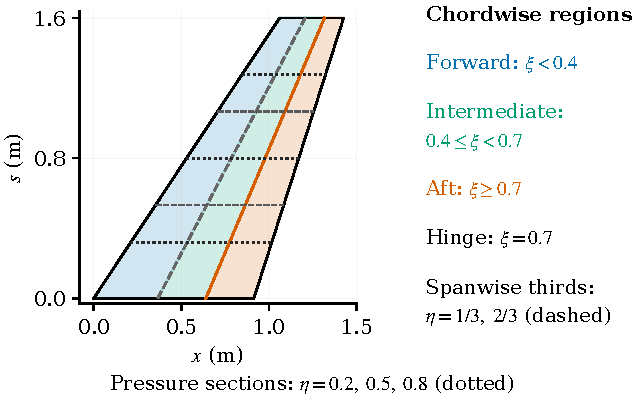
\includegraphics[width=.72\textwidth]{figures_revision_load_regions.pdf}
\caption{\DIFdelbeginFL \DIFdelFL{Undeformed reference }\DIFdelendFL \DIFaddbeginFL \DIFaddFL{Reference }\DIFaddendFL planform: chordwise \DIFdelbeginFL \DIFdelFL{integration }\DIFdelendFL \DIFaddbeginFL \DIFaddFL{loading }\DIFaddendFL regions, spanwise thirds, hinge, and pressure-section locations.}\label{fig:regions}\end{figure}

\label{anchor:reversal_definition}\DIFdelbegin \DIFdel{The local downstream direction must account for control rotation and surface orientation before reverse flow is assessed. Let }\DIFdelend \DIFaddbegin \DIFadd{For each surface face with unit normal $\mathbf n$, the downstream local chord direction }\DIFaddend $\mathbf d_c$ \DIFdelbegin \DIFdel{be the downstream chord direction: $(1,0,0)$ on the fixed panel, rotated about the physical hinge on the control. On each surface triangle with unit normal $\mathbf n$, its tangent-plane projection is normalized to give }\DIFdelend \DIFaddbegin \DIFadd{is rotated with the control, then projected into the tangent plane as }\DIFaddend $\mathbf t_c=[\mathbf d_c-(\mathbf d_c\cdot\mathbf n)\mathbf n]/\|\mathbf d_c-(\mathbf d_c\cdot\mathbf n)\mathbf n\|$. \DIFdelbegin \DIFdel{This construction points downstream on both physical sides, includes dihedral and flap rotation, and is applied after transforming symmetry-reflected states into the common physical convention}\DIFdelend \DIFaddbegin \DIFadd{Thus $C_{f,c}=\mathbf C_f\cdot\mathbf t_c$ measures the chordwise component of wall shear in the local, dihedral- and flap-aware orientation}\DIFaddend . End faces are excluded from \DIFdelbegin \DIFdel{the reverse-flow area calculation; the retained upper-control faces have no degenerate projected directions}\DIFdelend \DIFaddbegin \DIFadd{this shear diagnostic}\DIFaddend .

The \DIFdelbegin \DIFdel{signed coefficient $C_{f,c}=\mathbf C_f\cdot\mathbf t_c$ is negative where the chordwise component of wall shear points upstream, indicating local reverse flow. We report the }\DIFdelend fraction $f_{\mathrm{rev}}$ \DIFdelbegin \DIFdel{of the upper side of the deflected control }\DIFdelend \DIFaddbegin \DIFadd{is the upper-control area fraction }\DIFaddend ($\xi>0.7$, excluding end faces) \DIFdelbegin \DIFdel{satisfying }\DIFdelend \DIFaddbegin \DIFadd{with }\DIFaddend $C_{f,c}<0$\DIFdelbegin \DIFdel{, weighted by actual surface area. Thus $f_{\mathrm{rev}}=0.5$ }\DIFdelend \DIFaddbegin \DIFadd{. A value of 0.5 }\DIFaddend means that upstream-directed chordwise shear occupies half \DIFdelbegin \DIFdel{that upper-control area. Linear interpolation within each triangle locates the sign crossing. This area fraction measures the extent of reverse flow in the local chordwise direction near the wall. It is }\DIFdelend \DIFaddbegin \DIFadd{the control's upper surface. It indicates near-wall reversal, }\DIFaddend not a complete three-dimensional separation footprint\DIFdelbegin \DIFdel{: three-dimensional separation is characterized by the topology of the full skin-friction field~\mbox{%DIFAUXCMD
\cite{tobak1982topology}}\hskip0pt%DIFAUXCMD
, and on swept wings separation need not be accompanied by flow reversal~\mbox{%DIFAUXCMD
\cite{mccormack1949sweptforward}}\hskip0pt%DIFAUXCMD
. The scalar criterion therefore identifies one physically meaningful near-wall signature, without a topological analysis}\DIFdelend \DIFaddbegin \DIFadd{~\mbox{%DIFAUXCMD
\cite{tobak1982topology,mccormack1949sweptforward}}\hskip0pt%DIFAUXCMD
}\DIFaddend .

\label{end:sec:analysis}
\label{end:sec:methods}
\section{Experimental--Numerical Comparison}\label{sec:response}
\DIFdelbegin \DIFdel{The measurements establish whether lift and pitching moment change together as incidence rises at fixed control deflection. }\DIFdelend Figure~\ref{fig:measured} \DIFdelbegin \DIFdel{presents the reference zero-dihedral polars. The comparison includes deflections below and above the pronounced reduction in lift growth so that a change in moment response need not be assigned to the same incidenceor deflection as a lift feature}\DIFdelend \DIFaddbegin \DIFadd{compares the reference wind-tunnel lift and pitching moment over four control deflections. It shows whether their pre-stall changes coincide in incidence}\DIFaddend .

\begin{figure}[htbp]\centering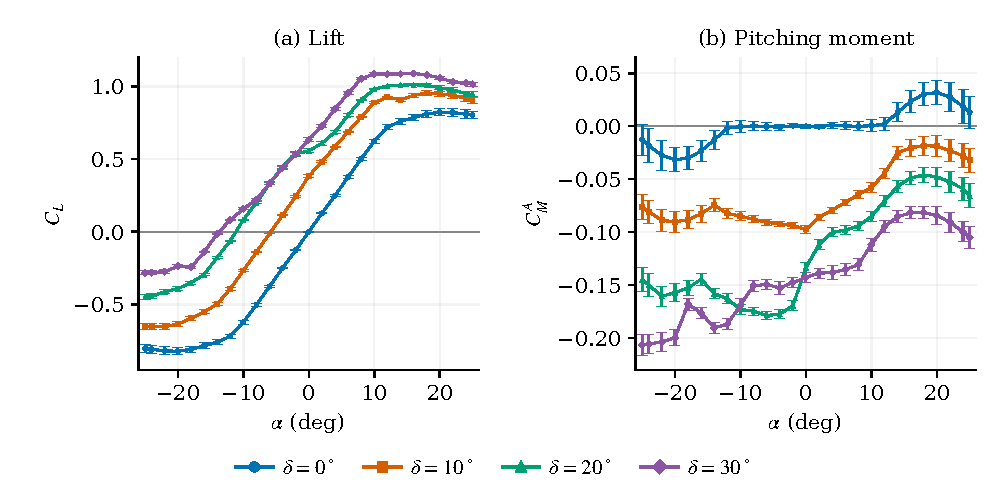
\includegraphics[width=\textwidth]{figures_revision_measured_baseline.pdf}
\caption{\DIFdelbeginFL \DIFdelFL{Experimental }\DIFdelendFL \DIFaddbeginFL \DIFaddFL{Reference wind-tunnel }\DIFaddendFL lift and \DIFdelbeginFL \DIFdelFL{pitching }\DIFdelendFL moment \DIFdelbeginFL \DIFdelFL{of the reference planform }\DIFdelendFL at zero dihedral\DIFdelbeginFL \DIFdelFL{for four control-surface deflections}\DIFdelendFL \DIFaddbeginFL \DIFaddFL{. Bars show propagated pointwise uncertainty; at $\delta=20\degc$, $\alpha=0\degc$, $u(C_L)\approx0.0133$}\DIFaddendFL .}\label{fig:measured}\end{figure}

\label{anchor:uncertainty}For configuration I at $\delta=20\degc$, the lift-coefficient increase over $\alpha=-2\to0\degc$ is approximately 0.020, compared with 0.089 over the preceding $\alpha=-4\to-2\degc$ interval. This is a roughly 78\% reduction in the interval's lift increase, while lift itself continues rising. Moment about the corresponding experimental aerodynamic center increases by $+0.036$, becoming less negative. Both departures in Table~\ref{tab:wt}, calculated against $\alpha\in\{-6,-4,-2\}\degc$, exceed the supplied-uncertainty sensitivities. The pointwise lift and moment uncertainty magnitudes are approximately 0.013 and 0.0046--0.0047, respectively; the local incidence spacing is $\Delta\alpha=2\degc$.

\begin{table}[htbp]\centering\small
\caption{Reference zero-dihedral measured lift and moment departures at $\delta=20\degc$, with their uncertainty sensitivities.}\label{tab:wt}
\begin{tabular}{llrrrr}\toprule
Geom., $\Gamma$, $\delta$ & Coefficient & $\alpha$ interval (deg) & $D$ & $u_{\mathrm{ind}}$ & $u_{\mathrm{L1}}$ \\\midrule
\tablerows{tables_revision_wt_reference_rows}
\bottomrule\end{tabular}\end{table}

The two coefficients respond differently at the lower deflection of $\delta=10\degc$: the measured moment change is $-0.0038$ over $\alpha=-2\to0\degc$ and $+0.011$ over $\alpha=0\to2\degc$, below the deflection that gives the pronounced $\delta=20\degc$ reduction in lift growth. At $\delta=30\degc$, the early lift feature is broader. The lift-coefficient increases are 0.077, 0.064, and 0.111 over $\alpha=-12\to-10\degc$, $\alpha=-10\to-8\degc$, and $\alpha=-8\to-6\degc$, while moment increases by about 0.018 on each of the first two intervals. Curvature of the preceding lift sequence makes the departure sensitive to the fitting range, so these actual interval changes describe the early feature more directly.

\FloatBarrier
\label{anchor:comparison}\DIFdelbegin \DIFdel{The numerical comparisons now assess separately the lift and moment evidence available for local interpretation. In Fig.~\ref{fig:comparison} , filled /solid and open/dashed curves denote WT and RANS , }\DIFdelend \DIFaddbegin \DIFadd{Figure~\ref{fig:comparison} compares WT (filled symbols, solid lines) with RANS (open symbols, dashed lines); }\DIFaddend circles and squares distinguish $\delta=20\degc$ and \DIFdelbegin \DIFdel{$\delta=30\degc$ deflections, and open diamonds mark zero-incidence numerical values. Grey bands mark }\DIFdelend \DIFaddbegin \DIFadd{$30\degc$. Plain and hatched grey bands indicate }\DIFaddend selected measured incidence intervals, \DIFdelbegin \DIFdel{plain for $\delta=20\degc$ and hatched for $\delta=30\degc$. They are neither uncertainty bands nor exact separation-onset locations. Each }\DIFdelend \DIFaddbegin \DIFadd{not uncertainty bands or precisely determined onset angles. Moments use each }\DIFaddend dataset's \DIFdelbegin \DIFdel{moment is about its corresponding }\DIFdelend aerodynamic center.

\begin{figure}[htbp]\centering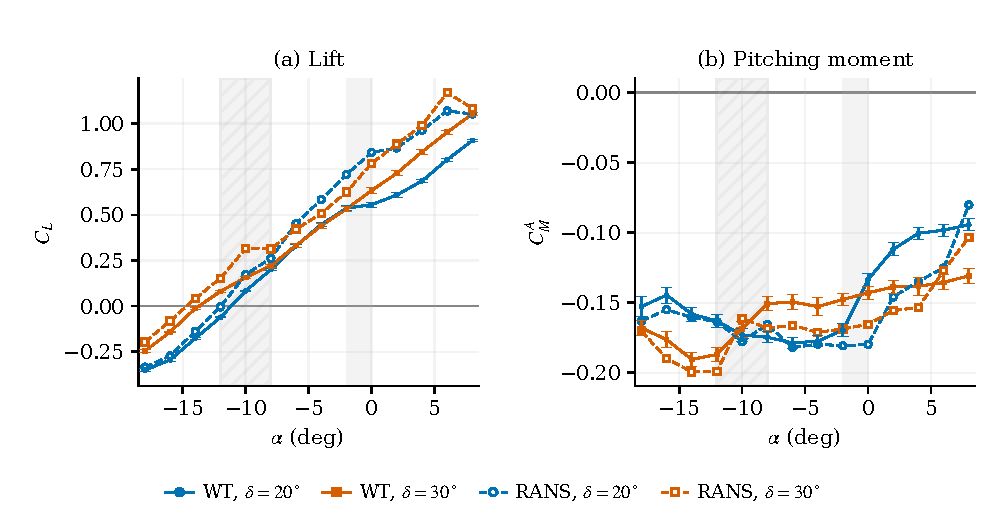
\includegraphics[width=\textwidth]{figures_revision_comparison.pdf}
\caption{Reference \DIFdelbeginFL \DIFdelFL{at zero dihedral: WT and RANS }\DIFdelendFL \DIFaddbeginFL \DIFaddFL{WT--RANS }\DIFaddendFL lift and \DIFdelbeginFL \DIFdelFL{pitching }\DIFdelendFL moment. \DIFdelbeginFL \DIFdelFL{Grey }\DIFdelendFL \DIFaddbeginFL \DIFaddFL{WT bars show propagated pointwise uncertainties; plain and hatched grey }\DIFaddendFL bands \DIFdelbeginFL \DIFdelFL{: }\DIFdelendFL \DIFaddbeginFL \DIFaddFL{mark }\DIFaddendFL measured intervals \DIFdelbeginFL \DIFdelFL{, plain }\DIFdelendFL \DIFaddbeginFL \DIFaddFL{at }\DIFaddendFL $\delta=20\degc$ \DIFdelbeginFL \DIFdelFL{, hatched $\delta=30\degc$}\DIFdelendFL \DIFaddbeginFL \DIFaddFL{and $30\degc$}\DIFaddendFL .}\label{fig:comparison}\end{figure}

For the reference model at $\delta = 20\degc$, the computed reduction in lift growth occurs over $\alpha=0\to2\degc$, one sampled interval later than in WT. The numerical zero-incidence lift is approximately 0.842, compared with WT 0.556 and uncertainty magnitude 0.013. A qualitatively similar reduction in lift growth and less-negative moment thus coexist with a substantial lift-level bias. At $\delta = 30\degc$, the early numerical lift change is sharper than the broad measured feature, and the moment departure depends more strongly on the preceding fitting range.

The \DIFdelbegin \DIFdel{reference computation captures the principal lift and pitching-moment trends. Sec.~\ref{sec:geometry_effects} presents comparisons with different geometries and their loading analysis. The following reference analysis investigates the computed loading changes themselves, using the integrated comparison to delimit their experimental interpretation}\DIFdelend \DIFaddbegin \DIFadd{following analysis therefore explains the computed reference loads, rather than assuming that partial agreement of integrated coefficients validates the local flow}\DIFaddend .
\FloatBarrier
\label{end:sec:response}
\section{Load Breakdown of the Reference Model}\label{sec:joint}
\subsection{Fixed-surface and control-surface loads}\label{sec:budget}
\DIFdelbegin \DIFdel{The reference analysis concerns }\DIFdelend \DIFaddbegin \DIFadd{For }\DIFaddend configuration I at \DIFdelbegin \DIFdel{zero dihedral and }\DIFdelend \DIFaddbegin \DIFadd{$\Gamma=0\degc$, }\DIFaddend $\delta=20\degc$\DIFdelbegin \DIFdel{. In }\DIFdelend \DIFaddbegin \DIFadd{, }\DIFaddend Fig.~\ref{fig:budget} \DIFdelbegin \DIFdel{, the upper panels show the fixed, control, and total coefficients. Dashed segments continue each preceding fitted slope, anchored at its actual zero-incidence value, across the shaded }\DIFdelend \DIFaddbegin \DIFadd{continues the fitted preceding incidence trends across }\DIFaddend $\alpha=0\to2\degc$ \DIFdelbegin \DIFdel{interval. The endpoint gap is the departure; the lower signed markers distinguish the actual increment from that departure. The two displays answer different questions: whether a surface gains load, and how its growth differs from the preceding trend}\DIFdelend \DIFaddbegin \DIFadd{(dashed). Endpoint gaps give the departures; the signed markers below distinguish actual increments from those departures}\DIFaddend .

\begin{figure}[htbp]\centering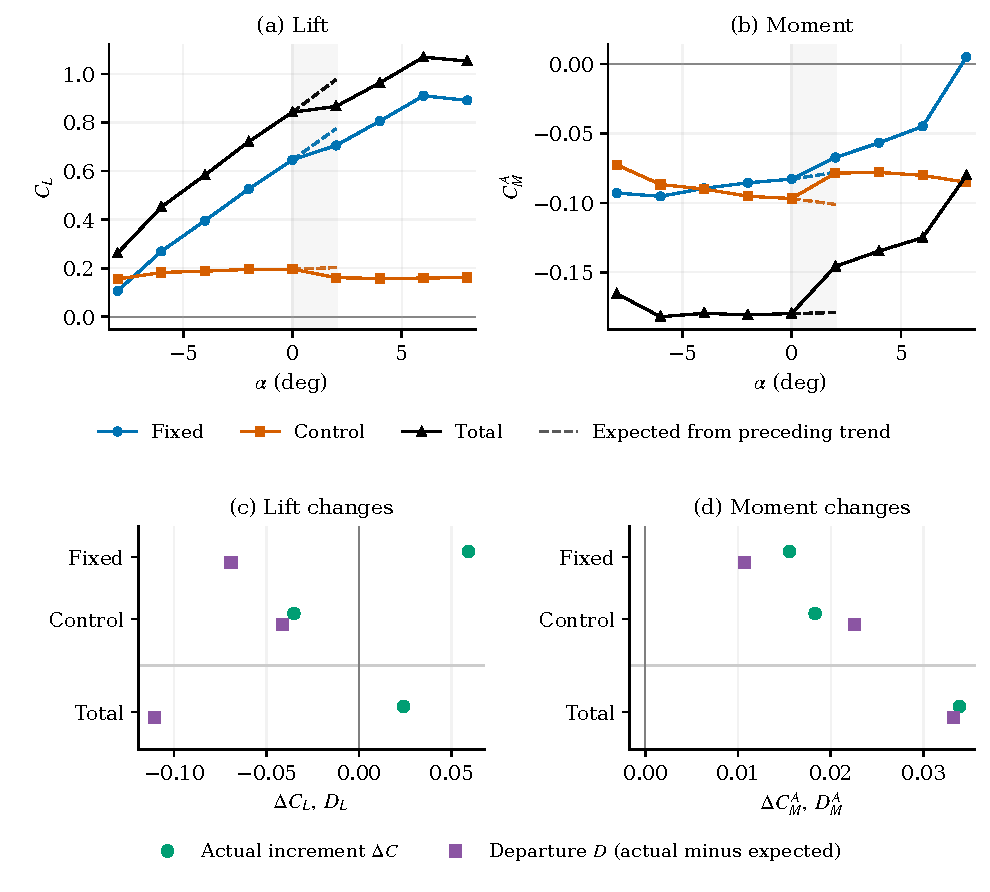
\includegraphics[width=\textwidth]{figures_revision_baseline_budget.pdf}
\caption{Fixed-surface, control-surface, and total numerical loading, with actual increments and departures from preceding incidence trends.}\label{fig:budget}\end{figure}

\DIFdelbegin \DIFdel{The fixed surface actually }\DIFdelend \DIFaddbegin \DIFadd{Over $\alpha=0\to2\degc$ the fixed surface }\DIFaddend gains $+0.0593$ in \DIFdelbegin \DIFdel{lift coefficient}\DIFdelend \DIFaddbegin \DIFadd{$C_L$}\DIFaddend , while the control loses $-0.0351$\DIFdelbegin \DIFdel{. Together, they yield }\DIFdelend \DIFaddbegin \DIFadd{, leaving }\DIFaddend a positive total \DIFdelbegin \DIFdel{increase }\DIFdelend \DIFaddbegin \DIFadd{increment }\DIFaddend of $+0.0242$. \DIFdelbegin \DIFdel{Continued growth of total lift is therefore sustained by the fixed-surface gain exceeding the control loss. Nevertheless, the fixed-surface gain is smaller than expected from its preceding slope, and both surfaces contribute negative departures: $-0.0692$ for fixed and $-0.0414$ for control, for a total of $-0.1106$ }\DIFdelend \DIFaddbegin \DIFadd{Nevertheless, both contribute to the shortfall against preceding lift-growth trends: $D_{L,\mathrm{fixed}}=-0.0692$ and $D_{L,\mathrm{control}}=-0.0414$, giving $D_{L,\mathrm{total}}=-0.1106$ }\DIFaddend (Table~\ref{tab:budget}). The \DIFdelbegin \DIFdel{reduction in lift growth therefore involves both the fixed surface and the control.
}%DIFDELCMD < 

%DIFDELCMD < %%%
\DIFdel{The fixed-surface share of }\DIFdelend \DIFaddbegin \DIFadd{fixed contribution represents }\DIFaddend approximately 63\% \DIFdelbegin \DIFdel{is the ratio $D_{L,\mathrm{fixed}}/D_{L,\mathrm{total}}$, using these two negative departures. It measures each surface's share of the computed lift-growth shortfall. Across the tested }\DIFdelend \DIFaddbegin \DIFadd{of that shortfall; across neighboring }\DIFaddend preceding-incidence \DIFdelbegin \DIFdel{ranges, this fraction }\DIFdelend \DIFaddbegin \DIFadd{fits it }\DIFaddend remains 62.4--62.6\% \DIFdelbegin \DIFdel{, while the total lift departure varies from approximately $-0.105$ to $-0.137$ }\DIFdelend (Appendix~\ref{app:sensitivity}). \DIFdelbegin \DIFdel{The amplitude depends on the empirical preceding trend, but its division between surfaces is comparatively stable}\DIFdelend \DIFaddbegin \DIFadd{This numerical robustness concerns the allocation of a trend-dependent shortfall, not the absolute size of the load change or a statistical confidence interval. Both the ordinary increments and the fitted-trend departures are additive because the same coefficient reference and fitting samples are used for each surface}\DIFaddend .



\begin{table}[htbp]\centering\small
\caption{Reference zero-dihedral lift and aerodynamic-center moment departures from preceding incidence trends; total includes tip loads.}\label{tab:budget}
\begin{tabular}{llrrr}\toprule
Geom., $\delta$, $\alpha$ interval & Departure & Fixed & Control & Total \\\midrule
\tablerows{tables_revision_budget_rows_compact}
\bottomrule\end{tabular}\end{table}

\DIFdelbegin \DIFdel{Pitching moment }\DIFdelend \DIFaddbegin \DIFadd{The moment departures }\DIFaddend about the numerical aerodynamic center \DIFdelbegin \DIFdel{has different relative contributions from the fixed and control surfaces. The departures }\DIFdelend reinforce: $+0.0107$ from the fixed surface and $+0.0226$ from the control \DIFdelbegin \DIFdel{. The fixed surface supplies the larger }\DIFdelend \DIFaddbegin \DIFadd{(Table~\ref{tab:budget}). Thus the control dominates the moment departure although the fixed surface dominates the }\DIFaddend lift-growth \DIFdelbegin \DIFdel{deficit, but the control supplies the larger moment departure . Which contribution is larger }\DIFdelend \DIFaddbegin \DIFadd{shortfall. The ranking }\DIFaddend depends on the moment \DIFdelbegin \DIFdel{axis: at }\DIFdelend \DIFaddbegin \DIFadd{pole: about }\DIFaddend the original numerical origin \DIFdelbegin \DIFdel{, }\DIFdelend \DIFaddbegin \DIFadd{the }\DIFaddend fixed/control \DIFdelbegin \DIFdel{moment departures are $+0.0529/ +0.0474$, so the fixed contribution is larger. Reinforcement persists at both axes. Locating these changes along the chord and span is therefore necessary to understand the combined force and moment response}\DIFdelend \DIFaddbegin \DIFadd{departures are $+0.0529/+0.0474$, still reinforcing. Their spatial distribution explains the difference}\DIFaddend .

Tip loads \DIFdelbegin \DIFdel{contribute less than 0.09\% of the changes listed in Table~\ref{tab:budget} and }\DIFdelend are included in \DIFdelbegin \DIFdel{the totals. The dihedral load decomposition retains their appreciable contribution }\DIFdelend \DIFaddbegin \DIFadd{all totals; their contributions in these reference intervals are below 0.09\%, but the dihedral moment analysis retains them }\DIFaddend explicitly.
\label{end:sec:budget}
\subsection{Pressure distribution and pitching moment}\label{sec:pressure}
Figure~\ref{fig:cp} \DIFdelbegin \DIFdel{first resolves the local pressure change between the actual }\DIFdelend \DIFaddbegin \DIFadd{compares pressure at }\DIFaddend $\alpha=0\degc$ and \DIFdelbegin \DIFdel{$\alpha=2\degc$ solutions in the reference load decomposition. Upper and lower sides are overlaid: solid curves with filled markers denote the upper side, and dotted curves with open markers denote the lower side. Circles and squares distinguish incidence. Upper leading-edge }\DIFdelend \DIFaddbegin \DIFadd{$2\degc$ on both sides of the reference wing at three span stations. Leading-edge }\DIFaddend suction strengthens, while the \DIFdelbegin \DIFdel{suction peak }\DIFdelend \DIFaddbegin \DIFadd{upper-side suction minimum }\DIFaddend near the hinge \DIFdelbegin \DIFdel{weakens}\DIFdelend \DIFaddbegin \DIFadd{becomes weaker}\DIFaddend . Here, pressure recovery \DIFdelbegin \DIFdel{denotes}%DIFDELCMD < \label{anchor:pressure_recovery} %%%
\DIFdelend \DIFaddbegin \DIFadd{means }\DIFaddend the chordwise rise \DIFdelbegin \DIFdel{downstream of the hinge suction }\DIFdelend \DIFaddbegin \DIFadd{in pressure downstream of that hinge-region }\DIFaddend minimum. The \DIFdelbegin \DIFdel{change in pressure recovery, together with the stronger }\DIFdelend \DIFaddbegin \DIFadd{increased }\DIFaddend leading-edge suction \DIFdelbegin \DIFdel{, redistributes loading along the chord}\DIFdelend \DIFaddbegin \DIFadd{alone might suggest stronger fixed-surface loading, but it does not establish how the *integrated* lift growth changes: suction can strengthen near the leading edge while loading elsewhere on the fixed chord stagnates or decreases. The chordwise lift contributions quantify the balance that cannot be inferred from isolated pressure peaks}\DIFaddend .

\begin{figure}[htbp]\centering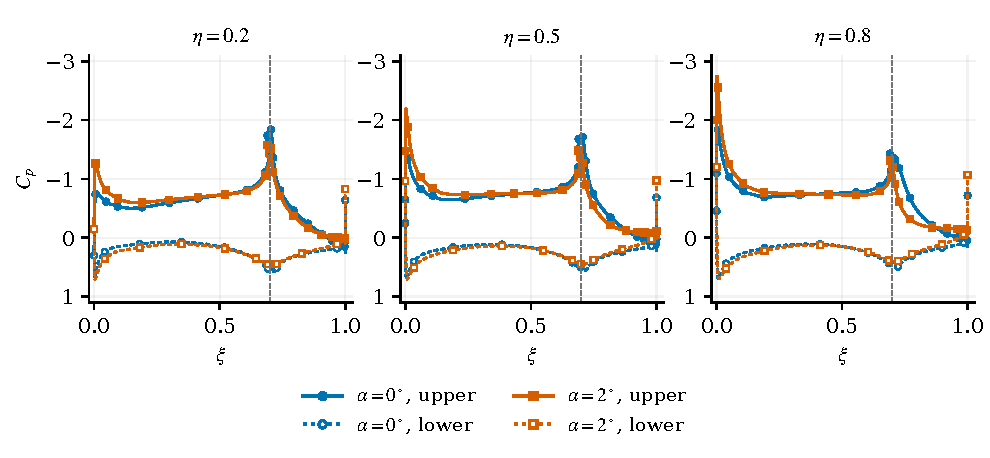
\includegraphics[width=\textwidth]{figures_revision_pressure_sections.pdf}
\caption{Chordwise pressure distributions at three span locations across the reference pre-stall loading change.}\label{fig:cp}\end{figure}

\DIFdelbegin \DIFdel{Figure~\ref{fig:spatial}(a) makes the connection to growth by integrating each chord region }\DIFdelend \DIFaddbegin \DIFadd{Summed }\DIFaddend over the semispan\DIFdelbegin \DIFdel{and comparing actual with expected lift increments. The forward region }\DIFdelend \DIFaddbegin \DIFadd{, the forward chord ($\xi<0.4$) }\DIFaddend gains $+0.0671$ \DIFdelbegin \DIFdel{, consistent with stronger leading-edge suction, but its preceding slope predicts $+0.1027$; it departs by }\DIFdelend \DIFaddbegin \DIFadd{in lift coefficient, but less than the expected $+0.1027$ from its preceding trend; its departure is }\DIFaddend $-0.0357$ \DIFaddbegin \DIFadd{(Fig.~\ref{fig:spatial}a)}\DIFaddend . The intermediate \DIFdelbegin \DIFdel{fixed-chord region }\DIFdelend \DIFaddbegin \DIFadd{fixed chord }\DIFaddend instead loses $-0.0097$ rather than gaining \DIFdelbegin \DIFdel{the expected }\DIFdelend $+0.0257$, \DIFdelbegin \DIFdel{giving a departure of }\DIFdelend \DIFaddbegin \DIFadd{departing by }\DIFaddend $-0.0354$. 
\DIFdelbegin \DIFdel{Stronger suction near the leading edge therefore coexists with both reduced forward-region growth and an actual intermediate-region loss. Together, these effects explain why the complete fixed surface still gains lift while strongly reducing lift growth in Fig.~\ref{fig:budget}.
}\DIFdelend 

The aft region loses $-0.0332$, compared with an expected $+0.0063$, giving a departure of $-0.0396$. Pressure \DIFdelbegin \DIFdel{supplies nearly all the principal lift departure, while viscous forces remain included in the integration}\DIFdelend \DIFaddbegin \DIFadd{forces account for nearly all of the lift-growth shortfall, with viscous contributions retained in the totals}\DIFaddend .

\begin{figure}[htbp]\centering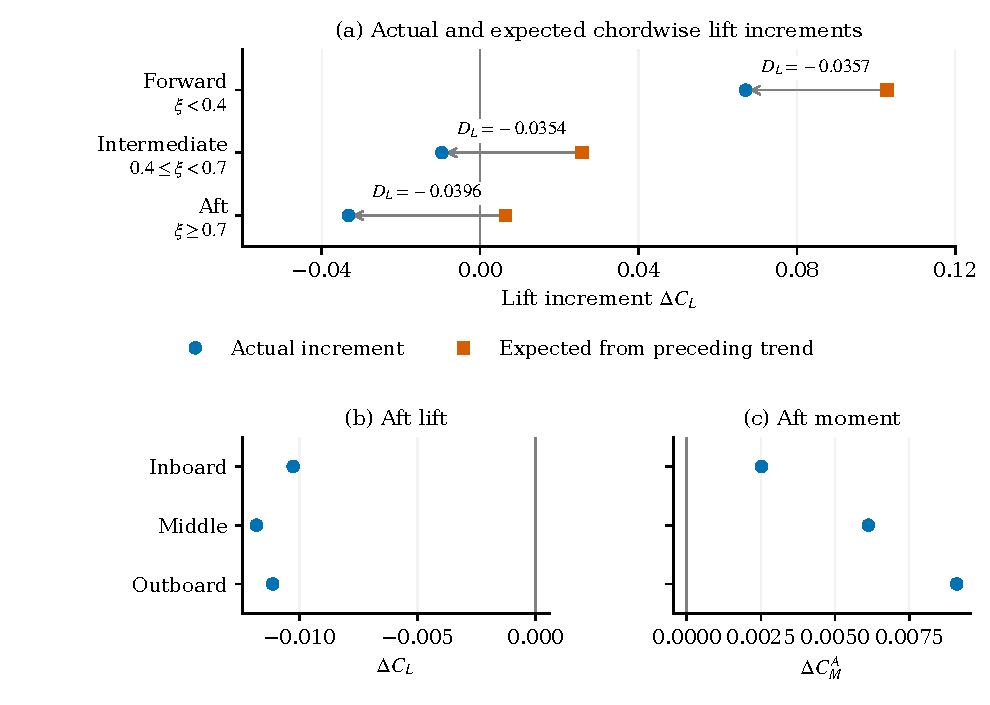
\includegraphics[width=\textwidth]{figures_revision_spatial_changes.pdf}
\caption{Chordwise and spanwise contributions to reference lift and pitching-moment changes over the selected pre-stall interval.}\label{fig:spatial}\end{figure}

\DIFdelbegin \DIFdel{Panels (b, c) answer a different question from panel (a): they show actual aft-region }\DIFdelend \DIFaddbegin \DIFadd{Across the inboard, middle, and outboard thirds of the aft chord, actual lift increments are similar }\DIFaddend (\DIFdelbegin \DIFdel{$\xi\geq0.7$) lift and moment increments in three spanwise regions, with no preceding-trend subtraction. The aft lift changes are similar , $-0.0103$, $-0.0118$, and $-0.0111$ from inboard to outboard, yet moment changes increase from $+0.00252$ through $+0.00612$ to $+0.00910$. The aft-swept geometry in }\DIFdelend \DIFaddbegin \DIFadd{$-0.0103,-0.0118,-0.0111$), but corresponding moment increments grow ($+0.00252,+0.00612,+0.00910$; }\DIFaddend Fig.~\DIFdelbegin \DIFdel{\ref{fig:regions} }\DIFdelend \DIFaddbegin \DIFadd{\ref{fig:spatial}b,c). The aft-swept planform }\DIFaddend places outboard aft loading farther downstream of the \DIFdelbegin \DIFdel{numerical }\DIFdelend aerodynamic center. \DIFdelbegin \DIFdel{For a local decrease in upward body-normal force, the factor $-(x-x_A)\,dF_z$ gives a positive moment change, larger for a longer downstream arm . The integrated }\DIFdelend \DIFaddbegin \DIFadd{Its longer $x-x_A$ arm makes comparable losses of upward }\DIFaddend body-normal force \DIFdelbegin \DIFdel{decreases in all three aft spanwise regions, supporting this interpretation; their detailed chordwise redistribution also enters the integral. The $F_x$ moment term }\DIFdelend \DIFaddbegin \DIFadd{produce greater nose-up moment changes through $-(x-x_A)dF_z$; the included }\DIFaddend $z\,dF_x$ \DIFdelbegin \DIFdel{remains included and is small here. The longer outboard arms therefore turn comparable aft lift losses into progressively larger positive moment increments .
}\DIFdelend \DIFaddbegin \DIFadd{term is small in this reference case. These are actual increments between computed states, not departures from the extrapolated baseline used in the chordwise shortfall comparison. Hence the chordwise and spanwise analyses explain complementary aspects of the response: the former identifies where the unexpected reduction in lift growth occurs, and the latter why the resulting force change carries different pitching-moment weight along the span.
}\DIFaddend \label{end:sec:pressure}
\subsection{Skin friction and reverse flow}\label{sec:reversal}
\DIFdelbegin \DIFdel{We can now compare the pressure and load changes with the evolution of near-wall flow on the deflected control.
}\DIFdelend Figure~\ref{fig:reversal} \DIFdelbegin \DIFdel{reports the proportion of its upper surface on which chordwise wall shearpoints upstream, using the definition in Sec.~\ref{sec:analysis}. Only the primary $C_{f,c}<0$ measure is plotted. The }\DIFdelend \DIFaddbegin \DIFadd{tracks the upper-control area fraction with upstream-directed chordwise shear; the }\DIFaddend open diamond marks \DIFaddbegin \DIFadd{the }\DIFaddend $\alpha=0\degc$ \DIFdelbegin \DIFdel{, the start of the interval examined in the surface maps and load analysis}\DIFdelend \DIFaddbegin \DIFadd{reference state}\DIFaddend .

\begin{figure}[htbp]\centering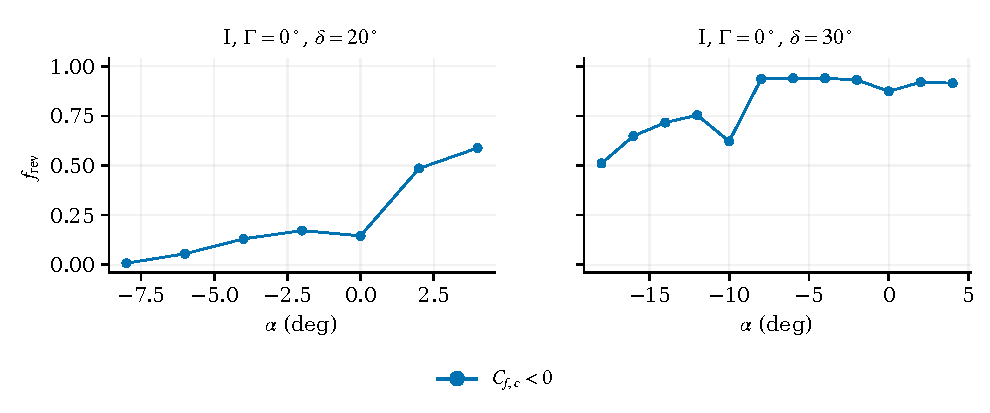
\includegraphics[width=.90\textwidth]{figures_revision_reversal.pdf}
\caption{Reference zero-dihedral upper control surface area fraction with reverse flow at $\delta=20\degc$ and $\delta=30\degc$.}\label{fig:reversal}\end{figure}

\DIFdelbegin \DIFdel{For the reference }\DIFdelend \DIFaddbegin \DIFadd{At }\DIFaddend $\delta=20\degc$\DIFdelbegin \DIFdel{calculation, that area fraction grows from about 15\% to 49\% ($0.146$ to $0.485$) }\DIFdelend \DIFaddbegin \DIFadd{, this fraction rises from 0.146 to 0.485 }\DIFaddend across $\alpha=0\to2\degc$, \DIFdelbegin \DIFdel{the same interval as the reduced fixed-surface growth, control lift loss }\DIFdelend \DIFaddbegin \DIFadd{coinciding with the computed lift-growth shortfall }\DIFaddend and positive moment change. \DIFdelbegin \DIFdel{The maps in Fig.~\ref{fig:transition} distinguish this area increase from a change in location.
}%DIFDELCMD < 

%DIFDELCMD < %%%
\DIFdelend Figure~\ref{fig:transition} shows \DIFdelbegin \DIFdel{the signed coefficient}%DIFDELCMD < \label{anchor:local_shear} %%%
\DIFdel{$C_{f,c}$ on the upper surface for both reference deflections, using identical projections and color scales. At $\delta=20\degc$, the $\alpha=0\degc$ state has a narrow region of reverse flow adjacent to the hinge, followed by predominantly downstream shear.
At $\alpha=2\degc$, the main region of reverse flow instead lies near the trailing edge. At $\alpha=4\degc$, this region of reverse flow near }\DIFdelend \DIFaddbegin \DIFadd{that the reversed-shear region also changes location.
}

\DIFadd{At $\alpha=0\degc$, reverse chordwise shear lies chiefly near the hinge; at $2\degc$ it is concentrated toward }\DIFaddend the trailing edge\DIFdelbegin \DIFdel{extends farther upstream . The change across $\alpha=0\to2\degc$ therefore includes a change in the location of reverse flow, alongside the }\DIFdelend \DIFaddbegin \DIFadd{, and by $4\degc$ extends upstream (Fig.~\ref{fig:transition}). Thus the increase in the upper-control reversed-shear area across the key interval does not represent uniform growth of the original hinge-adjacent zone. This evolving near-wall pattern accompanies }\DIFaddend weakened hinge suction and \DIFdelbegin \DIFdel{aft load loss in Figs. ~\ref{fig:cp} and \ref{fig:spatial}; it is not simply uniform growth of }\DIFdelend \DIFaddbegin \DIFadd{reduced aft loading in }\DIFaddend the \DIFdelbegin \DIFdel{initial hinge-adjacent band}\DIFdelend \DIFaddbegin \DIFadd{surface-force contributions. Its spatial development is informative even though the sign of a single wall-shear component cannot uniquely identify the full three-dimensional separation topology}\DIFaddend .

\DIFdelbegin \DIFdel{By $\alpha=4\degc$, }\DIFdelend \DIFaddbegin \DIFadd{At $4\degc$, the reversed-shear fraction reaches }\DIFaddend about 59\%\DIFdelbegin \DIFdel{of the upper control experiences reverse flow, while the total lift increase }\DIFdelend \DIFaddbegin \DIFadd{, even though total lift grows more }\DIFaddend over $\alpha=2\to4\degc$ \DIFdelbegin \DIFdel{is 0.0968, larger than the preceding 0.0242. Stronger total lift growth can thus coexist with a larger area of reverse flow because the integrated response combines the evolving loading on both surfaces. The extent of reverse flow characterizes near-wall flow, but does not by itself determine the pressure force or pitching moment}\DIFdelend \DIFaddbegin \DIFadd{($+0.0968$) than over $0\to2\degc$ ($+0.0242$). A larger reversal area need not imply a smaller total lift increment}\DIFaddend .

\begin{figure}[htbp]\centering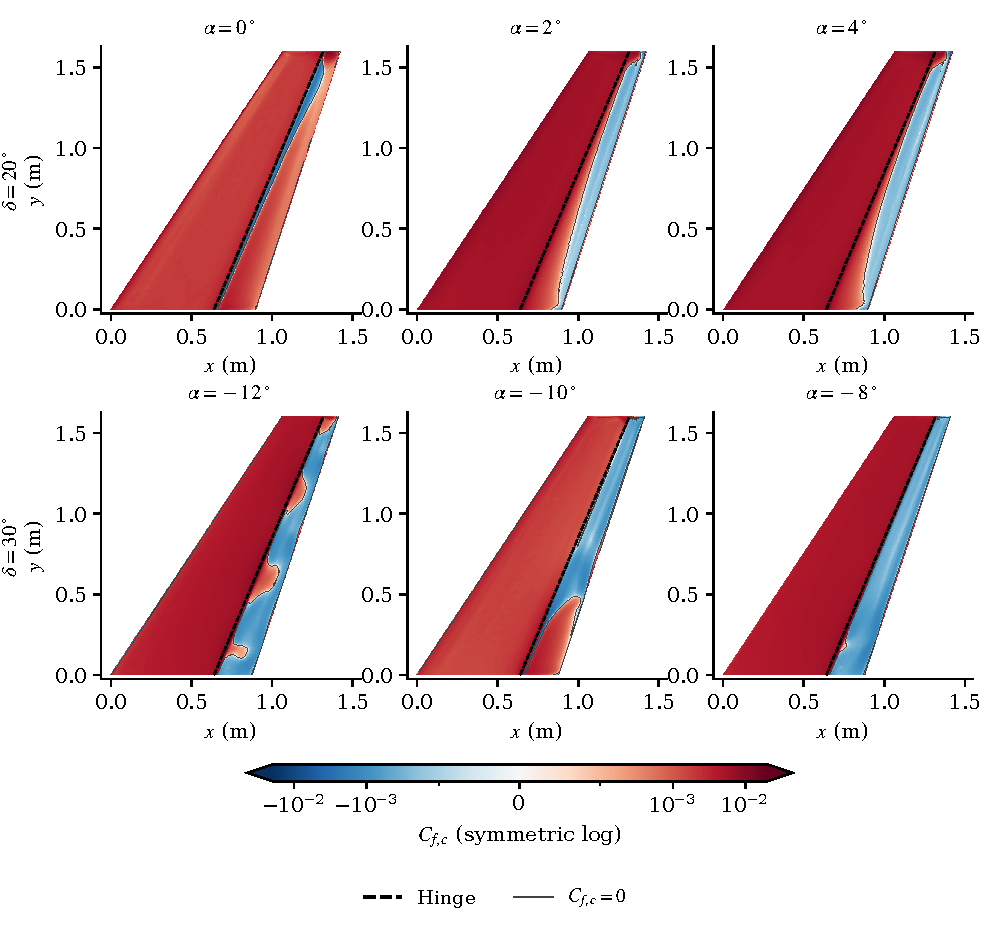
\includegraphics[width=\textwidth]{figures_revision_surface_sequence.pdf}
\caption{Reference upper-surface chordwise skin friction across the loading changes at $\delta=20\degc$ (top) and $\delta=30\degc$ (bottom) deflection.}\label{fig:transition}\end{figure}

At $\delta=30\degc$, the \DIFdelbegin \DIFdel{reference reduction in lift growth occurs much }\DIFdelend \DIFaddbegin \DIFadd{corresponding loading change occurs }\DIFaddend earlier, over $\alpha=-10\to-8\degc$\DIFdelbegin \DIFdel{. Fixed lift still increases }\DIFdelend \DIFaddbegin \DIFadd{: fixed-surface lift grows }\DIFaddend by $+0.0406$ \DIFdelbegin \DIFdel{, }\DIFdelend while the control loses $-0.0436$, \DIFdelbegin \DIFdel{leaving }\DIFdelend \DIFaddbegin \DIFadd{giving }\DIFaddend a small total decrease \DIFdelbegin \DIFdel{of }\DIFdelend \DIFaddbegin \DIFadd{(}\DIFaddend $-0.0030$\DIFdelbegin \DIFdel{. Both lift departures remain negative. The lower row of Fig.~\ref{fig:transition} follows this earlier interval. Over it, the upper control surface reverse-flow area }\DIFdelend \DIFaddbegin \DIFadd{). The reversed-shear }\DIFaddend fraction rises from \DIFdelbegin \DIFdel{approximately 62\% to 94\% ($0.622$ to $0.935$).The recurring association is thus reduced aft loading with expansion of the existing reverse-flow region, although the total lift increment changes sign because the fixed gain no longer outweighs the control loss}\DIFdelend \DIFaddbegin \DIFadd{0.622 to 0.935 over this interval (Fig.~\ref{fig:transition}, lower row)}\DIFaddend .

\DIFdelbegin \DIFdel{The moment result at $\delta=30\degc$ is different}\DIFdelend \DIFaddbegin \DIFadd{Unlike the reinforcing moment departures at $\delta=20\degc$, those at $30\degc$ partly cancel}\DIFaddend : the fixed-surface \DIFdelbegin \DIFdel{departure }\DIFdelend \DIFaddbegin \DIFadd{contribution }\DIFaddend is negative and the control \DIFdelbegin \DIFdel{departure positive, so they partly cancel (Table~\ref{tab:budget}). Across the tested preceding fitting ranges, }\DIFdelend \DIFaddbegin \DIFadd{contribution positive. The }\DIFaddend total moment departure \DIFdelbegin \DIFdel{varies from approximately }\DIFdelend \DIFaddbegin \DIFadd{ranges from }\DIFaddend $-0.0262$ to $+0.0076$ \DIFdelbegin \DIFdel{as the opposing contributions change their balance. Its total sign is therefore not robustto this empirical reference. This contrasts with the reinforcing moment departures at $\delta=20\degc$ and shows why reverse-flow }\DIFdelend \DIFaddbegin \DIFadd{across preceding-slope fits, so its sign is not robust. Taken together, the two deflections show why reversed-shear }\DIFaddend area alone cannot \DIFdelbegin \DIFdel{infer the sign of the integrated pitching response}\DIFdelend \DIFaddbegin \DIFadd{determine integrated lift or moment}\DIFaddend .
\FloatBarrier
\label{end:sec:joint}
\label{end:sec:reversal}
\section{\DIFdelbegin \DIFdel{Effects of }\DIFdelend Dihedral and \DIFdelbegin \DIFdel{Sweep}\DIFdelend \DIFaddbegin \DIFadd{Planform Dependence}\DIFaddend }\label{sec:geometry_effects}
\DIFdelbegin \DIFdel{The same component and regional load decomposition is now applied to the }\DIFdelend \DIFaddbegin \DIFadd{We next examine how }\DIFaddend dihedral and planform \DIFdelbegin \DIFdel{comparisons. We present their measured responses and WT--RANS correspondence alongside the numerical loading analysis}\DIFdelend \DIFaddbegin \DIFadd{geometry modify the fixed- and control-surface loads and their pitching-moment contributions, beginning with the measured and computed coefficients}\DIFaddend .

Table~\ref{tab:wt_geometry} \DIFdelbegin \DIFdel{reports }\DIFdelend \DIFaddbegin \DIFadd{gives }\DIFaddend the measured departures and uncertainty sensitivities for these \DIFdelbegin \DIFdel{geometry comparisons, using the definitions in Sec.~\ref{sec:analysis}}\DIFdelend \DIFaddbegin \DIFadd{cases}\DIFaddend .

\begin{table}[htbp]\centering\small
\caption{Measured lift and moment departures for the dihedral and forward-swept cases, with their uncertainty sensitivities.}\label{tab:wt_geometry}
\begin{tabular}{llrrrr}\toprule
Geom., $\Gamma$, $\delta$ & Coefficient & $\alpha$ interval (deg) & $D$ & $u_{\mathrm{ind}}$ & $u_{\mathrm{L1}}$ \\\midrule
\tablerows{tables_revision_wt_geometry_rows}
\bottomrule\end{tabular}\end{table}

\subsection{Effect of dihedral}\label{sec:dihedral}
Figure~\ref{fig:comparison_dihedral} \DIFdelbegin \DIFdel{brings together the wind-tunnel dihedral comparison (upper panels) }\DIFdelend \DIFaddbegin \DIFadd{compares the dihedral WT polars }\DIFaddend and the $\Gamma=45\degc$ WT--RANS \DIFdelbegin \DIFdel{comparison (lower panels)}\DIFdelend \DIFaddbegin \DIFadd{response}\DIFaddend . At $\delta=20\degc$, measured lift growth remains suppressed \DIFdelbegin \DIFdel{across }\DIFdelend \DIFaddbegin \DIFadd{over }\DIFaddend $\alpha=-2\to2\degc$ \DIFdelbegin \DIFdel{, }\DIFdelend while the moment departure over \DIFdelbegin \DIFdel{$\alpha=-2\to0\degc$ is smaller than }\DIFdelend \DIFaddbegin \DIFadd{$-2\to0\degc$ is below }\DIFaddend both uncertainty sensitivities \DIFdelbegin \DIFdel{in }\DIFdelend \DIFaddbegin \DIFadd{(}\DIFaddend Table~\ref{tab:wt_geometry}\DIFaddbegin \DIFadd{)}\DIFaddend . At $\delta=30\degc$, \DIFdelbegin \DIFdel{the selected reduction in lift growth occurs over $\alpha=-2\to0\degc$, but the moment decreases earlier , by 0.027 over $\alpha=-4\to-2\degc$. That moment departure is comparable with $u_{\mathrm{ind}}$ and smaller than $u_{\mathrm{L1}}$. The joint response differs from the clearly resolved reference $\delta=20\degc$ }\DIFdelend lift \DIFdelbegin \DIFdel{/moment change}\DIFdelend \DIFaddbegin \DIFadd{growth decreases over $-2\to0\degc$, but moment falls earlier ($-0.027$ over $-4\to-2\degc$); its departure does not exceed the conservative uncertainty sensitivity}\DIFaddend .

\begin{figure}[htbp]\centering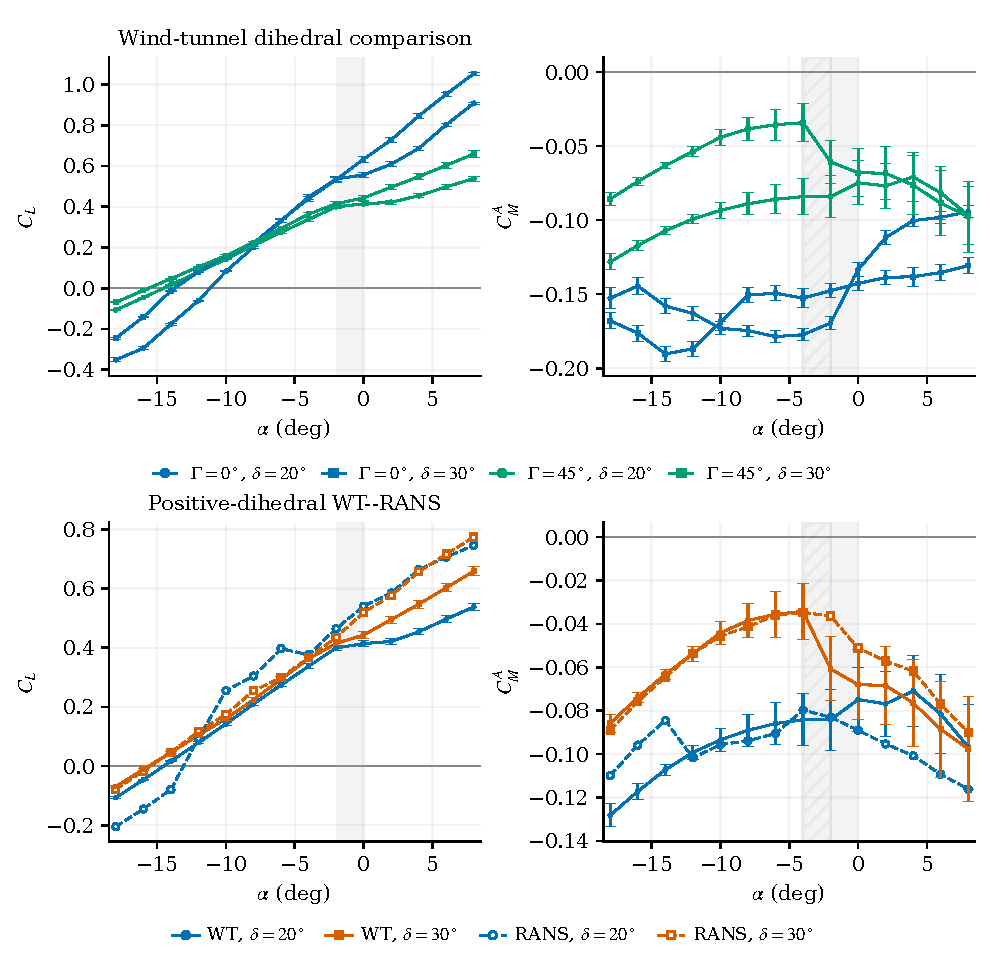
\includegraphics[width=\textwidth]{figures_revision_comparison_dihedral.pdf}
\caption{Wind-tunnel dihedral \DIFdelbeginFL \DIFdelFL{comparison (top) }\DIFdelendFL and positive-dihedral WT--RANS \DIFdelbeginFL \DIFdelFL{comparison (bottom)}\DIFdelendFL \DIFaddbeginFL \DIFaddFL{comparisons}\DIFaddendFL . \DIFdelbeginFL \DIFdelFL{Grey }\DIFdelendFL \DIFaddbeginFL \DIFaddFL{WT bars show propagated pointwise uncertainties; plain and hatched }\DIFaddendFL bands mark \DIFdelbeginFL \DIFdelFL{measured }\DIFdelendFL \DIFaddbeginFL \DIFaddFL{selected incidence }\DIFaddendFL intervals\DIFdelbeginFL \DIFdelFL{: plain $\delta=20\degc$, hatched $\delta=30\degc$}\DIFdelendFL .}\label{fig:comparison_dihedral}\end{figure}

\DIFdelbegin \DIFdel{The computed sequence has weaker correspondence with these }\DIFdelend \DIFaddbegin \DIFadd{RANS corresponds less closely to the dihedral }\DIFaddend measurements. At $\delta=20\degc$ \DIFdelbegin \DIFdel{, numerical lift decreases }\DIFdelend \DIFaddbegin \DIFadd{it predicts a lift decrease }\DIFaddend over $\alpha=-6\to-4\degc$ \DIFdelbegin \DIFdel{while measured lift increases; this earlier computed change, with a rise in the upper-control reverse-flow area fractionfrom 0.12 to 0.54, has no measured counterpart. At the incidences of }\DIFdelend \DIFaddbegin \DIFadd{absent from WT; that computed interval also has a marked increase in the control reversed-shear fraction. Near }\DIFaddend the measured feature, \DIFdelbegin \DIFdel{the computed lift increase falls }\DIFdelend \DIFaddbegin \DIFadd{by contrast, successive numerical lift increments decrease }\DIFaddend from 0.0763 \DIFdelbegin \DIFdel{over $\alpha=-2\to0\degc$ }\DIFdelend to 0.0444 over \DIFdelbegin \DIFdel{$\alpha=0\to2\degc$, while the reverse-flow area fraction grows from 0.49 to 0.58. RANS therefore reproduces a reduction in lift growth with expanding reverse flow on the control at these incidences, but not the sustained measured reduction over $\alpha=-2\to2\degc$ or its weak moment feature}\DIFdelend \DIFaddbegin \DIFadd{$-2\to0\degc$ and $0\to2\degc$, but the measured weak moment response is not reproduced}\DIFaddend . At $\delta=30\degc$, the \DIFdelbegin \DIFdel{negative numerical moment change occurs over $\alpha=-2\to0\degc$, one sampled }\DIFdelend \DIFaddbegin \DIFadd{computed moment decrease occurs one incidence }\DIFaddend interval later than \DIFdelbegin \DIFdel{the measuredchange}\DIFdelend \DIFaddbegin \DIFadd{measured}\DIFaddend . The following \DIFdelbegin \DIFdel{decomposition consequently concerns }\DIFdelend \DIFaddbegin \DIFadd{analysis identifies how }\DIFaddend the computed dihedral \DIFdelbegin \DIFdel{response}\DIFdelend \DIFaddbegin \DIFadd{loading changes contribute to pitching moment}\DIFaddend .

At $\alpha=0\degc$, $\delta=20\degc$, the computed \DIFdelbegin \DIFdel{lift coefficient is approximately }\DIFdelend \DIFaddbegin \DIFadd{$45\degc$-dihedral lift is }\DIFaddend 0.301 lower \DIFdelbegin \DIFdel{with $\Gamma=45\degc$. Projection of the reference }\DIFdelend \DIFaddbegin \DIFadd{than at zero dihedral. Projecting the zero-dihedral }\DIFaddend panel-normal loading onto the \DIFdelbegin \DIFdel{common lift direction}\DIFdelend \DIFaddbegin \DIFadd{inclined lift direction, without changing its magnitude, }\DIFaddend accounts algebraically for about 0.247 of \DIFdelbegin \DIFdel{this difference; changes in local loading and the spanwise-force contribution supply the remainder. The absolute lift difference therefore includes a substantial projection contribution, while the successive incidence increments require the separate load analysis }\DIFdelend \DIFaddbegin \DIFadd{the difference. The incidence-dependent response is examined separately }\DIFaddend below.

The computed \DIFdelbegin \DIFdel{lift increments change differently with incidenceon the two models. At the same }\DIFdelend \DIFaddbegin \DIFadd{ordering of lift increments reverses with incidence: at }\DIFaddend $\delta=20\degc$\DIFdelbegin \DIFdel{deflection, the actual lift increase over $\alpha=-2\to0\degc$ is }\DIFdelend \DIFaddbegin \DIFadd{, lift grows by }\DIFaddend 0.1210 \DIFdelbegin \DIFdel{at zero dihedral and }\DIFdelend \DIFaddbegin \DIFadd{($\Gamma=0\degc$) versus }\DIFaddend 0.0763 \DIFdelbegin \DIFdel{at $\Gamma=45\degc$. Across the next interval, $\alpha=0\to2\degc$, the ordering reverses: the increases are }\DIFdelend \DIFaddbegin \DIFadd{($45\degc$) over $\alpha=-2\to0\degc$, but by }\DIFaddend 0.0242 \DIFdelbegin \DIFdel{and }\DIFdelend \DIFaddbegin \DIFadd{versus }\DIFaddend 0.0444 \DIFdelbegin \DIFdel{. Although the dihedral model has lower absolute lift, it gains more lift over that latter interval. The change in ordering shows that the relative lift growth depends on incidence . Table~\ref{tab:geometry_budget} shows that the $\Gamma=45\degc$ }\DIFdelend \DIFaddbegin \DIFadd{over $0\to2\degc$. Thus dihedral does more than shift absolute lift; the relative *increment* changes with incidence and cannot be described by a fixed projection factor. For the latter interval, the $45\degc$ }\DIFaddend fixed surface still gains lift \DIFdelbegin \DIFdel{over $\alpha=0\to2\degc$, }\DIFdelend while the control loses \DIFdelbegin \DIFdel{lift. Its moment about its computed aerodynamic centerdecreases due to contributions from the fixed surface, control, and tip. The table retains the tip explicitly because its moment contribution is appreciable in these dihedral cases}\DIFdelend \DIFaddbegin \DIFadd{it (Table~\ref{tab:geometry_budget}), and all three surface groups contribute to its negative pitching-moment increment about its own aerodynamic center. The zero-dihedral model nevertheless retains the larger absolute lift in both states. Comparing increments isolates a different aspect of the response than comparing the lift levels at one incidence}\DIFaddend .

\begin{table}[htbp]\centering\small
\caption{Actual coefficient increments for the dihedral and forward-swept cases; moments are about their corresponding numerical aerodynamic centers.}\label{tab:geometry_budget}
\begin{tabular}{llrrrr}\toprule
Geom., $\Gamma$, $\delta$, $\alpha$ interval & Increment & Fixed & Control & Tip & Total \\\midrule
\tablerows{tables_revision_geometry_budget_rows}
\bottomrule\end{tabular}\end{table}

\DIFdelbegin \DIFdel{Pitching moment depends on where $F_x$ and $F_z$ act. Dihedral places }\DIFdelend \DIFaddbegin \DIFadd{Dihedral elevates }\DIFaddend the loading above the reference axis, \DIFdelbegin \DIFdel{so $F_x$ contributes through the vertical arm $z$. The $F_z$ contribution is weighted by the downstream arm $x-x_A$ (Eq. ~\ref{eq:moment}).Both numerical solutions are referred }\DIFdelend \DIFaddbegin \DIFadd{adding an axial-force moment through $z\,dF_x$, while the normal-force contribution uses $-(x-x_A)dF_z$. Because the moment pole affects a comparison of dihedral configurations~\mbox{%DIFAUXCMD
\cite{maggin1946dihedral}}\hskip0pt%DIFAUXCMD
, Fig.~\ref{fig:dihedral} transports both numerical cases }\DIFaddend to the same \DIFdelbegin \DIFdel{physical }\DIFdelend axis $A_I$. \DIFdelbegin \DIFdel{Maggin and Shanks~\mbox{%DIFAUXCMD
\cite{maggin1946dihedral} }\hskip0pt%DIFAUXCMD
showed why this choice matters: for a 40$\degc$ swept-back wing, moments about fixed reference axes indicated an apparent increase in longitudinal stability with geometric dihedral, whereas only a slight change remained when each configuration was referred to its own mean aerodynamic chord. The common axis therefore compares the loading and its moment arms about one physical point, whereas }\DIFdelend Table~\ref{tab:geometry_budget} \DIFaddbegin \DIFadd{instead }\DIFaddend uses each configuration's \DIFdelbegin \DIFdel{computed aerodynamic center. Figure~\ref{fig:dihedral}(a ,b) compares their moment increments through
}\DIFdelend \DIFaddbegin \DIFadd{own aerodynamic center; the corresponding component increments must not be subtracted without first accounting for this difference in reference. The fixed/control loads identify which surfaces contribute to the moment change; the common-axis balance distinguishes the axial- and normal-force contributions. For a matched incidence interval, the difference of those actual moment increments is
}\DIFaddend \begin{equation}
 \mathcal I_M=[C_{M,45}^{A_I}(\alpha_b)-C_{M,45}^{A_I}(\alpha_a)]
             -[C_{M,0}^{A_I}(\alpha_b)-C_{M,0}^{A_I}(\alpha_a)]
\label{eq:interval}
\end{equation}
A negative $\mathcal I_M$ means that the moment increase is smaller, or the decrease larger, with dihedral over the same incidence interval. These are differences of actual moment increments, not departures from preceding fitted trends.

\begin{figure}[htbp]\centering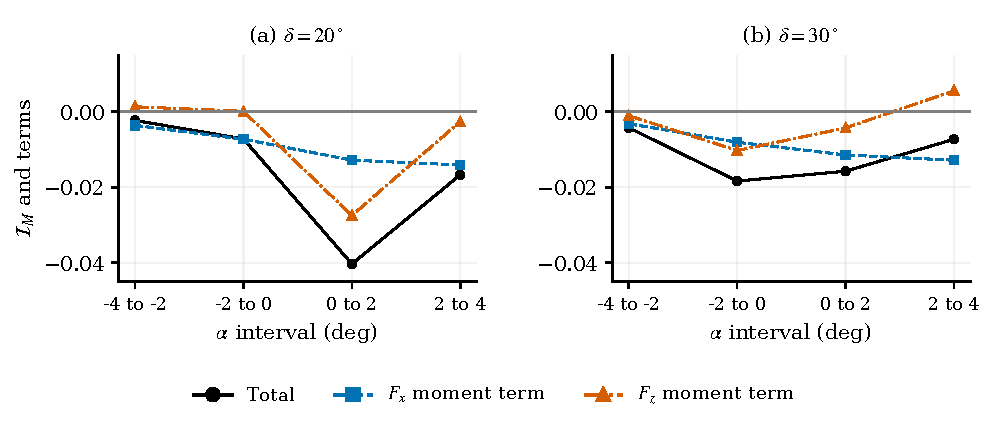
\includegraphics[width=\textwidth]{figures_revision_dihedral_intervals.pdf}
\caption{Dihedral differences in moment increments about the common axis $A_I$ and their $F_x$ and $F_z$ contributions: $\delta=20\degc$ (left) and $\delta=30\degc$ (right).}\label{fig:dihedral}\end{figure}

At $\delta=20\degc$, the \DIFdelbegin \DIFdel{$F_x$ moment term gives a negative difference in every plotted interval. Over }\DIFdelend \DIFaddbegin \DIFadd{force-moment differences partly compensate over }\DIFaddend $\alpha=-4\to-2\degc$ \DIFdelbegin \DIFdel{, it contributes }\DIFdelend \DIFaddbegin \DIFadd{(}\DIFaddend $-0.00362$ \DIFdelbegin \DIFdel{, partly offset by a }\DIFdelend \DIFaddbegin \DIFadd{from $F_x$, }\DIFaddend $+0.00131$ \DIFdelbegin \DIFdel{contribution }\DIFdelend from $F_z$\DIFdelbegin \DIFdel{, leaving $\mathcal I_M=-0.00231$. Across $\alpha=0\to2\degc$, the terms instead reinforce : }\DIFdelend \DIFaddbegin \DIFadd{), but reinforce over $0\to2\degc$ (}\DIFaddend $-0.01283$ \DIFdelbegin \DIFdel{from $F_x$ }\DIFdelend and $-0.02750$\DIFdelbegin \DIFdel{from $F_z$ give $-0.04033$. The $F_z$ moment term supplies the larger difference during this reference loading change. Over $\alpha=2\to4\degc$, its contribution falls to $-0.00260$, while the contribution from $F_x$ remains $-0.01412$ and dominates the $-0.01672$ total. A single relative weighting of the two moment terms therefore cannot describe the sequence}\DIFdelend \DIFaddbegin \DIFadd{, total $\mathcal I_M=-0.04033$). The larger normal-force contribution in the latter interval reflects changes in both loading and its streamwise moment arm, which cannot be inferred from a fixed lift-projection factor (Fig.~\ref{fig:dihedral})}\DIFaddend .

At $\delta=30\degc$, the \DIFdelbegin \DIFdel{terms }\DIFdelend \DIFaddbegin \DIFadd{axial- and normal-force terms also }\DIFaddend reinforce over $\alpha=-2\to0\degc$\DIFdelbegin \DIFdel{: $-0.00808$ from $F_x$ and $-0.01027$ from $F_z$ give a total $-0.01836$. Over $\alpha=0\to2\degc$, both remain negative, with the $F_x$ contribution larger. Over $\alpha=2\to4\degc$, a positive difference from $F_z$ }\DIFdelend \DIFaddbegin \DIFadd{, producing a moment-increment difference }\DIFaddend of \DIFdelbegin \DIFdel{$+0.00556$ offsets part of the $-0.01286$ difference from $F_x$, leaving $-0.00730$. This change from reinforcement to compensation concerns the moment-term differences between geometries; it is distinct from fixed/control moment-departure reinforcement in Sec.~\ref{sec:budget}}\DIFdelend \DIFaddbegin \DIFadd{$-0.01836$. The relative contributions thus reflect the incidence-dependent forces and their moment arms, rather than a constant geometric scaling}\DIFaddend .

The \DIFdelbegin \DIFdel{next step is to establish whether these moment changes accompany expansion of reverse flow on the control or loading changes elsewhere on the model. At }\DIFdelend $\delta=30\degc$ \DIFdelbegin \DIFdel{, the }\DIFdelend \DIFaddbegin \DIFadd{moment decrease occurs while }\DIFaddend upper-control \DIFdelbegin \DIFdel{reverse-flow area fraction is already }\DIFdelend \DIFaddbegin \DIFadd{reversed-shear area changes little: }\DIFaddend 0.889\DIFdelbegin \DIFdel{at $\alpha=-2\degc$, increasing only to }\DIFdelend \DIFaddbegin \DIFadd{, }\DIFaddend 0.911 and 0.912 at \DIFdelbegin \DIFdel{$\alpha=0\degc$ and $\alpha=2\degc$ }\DIFdelend \DIFaddbegin \DIFadd{$\alpha=-2,0,2\degc$ }\DIFaddend (Fig.~\ref{fig:reversal_geometry}). Over \DIFdelbegin \DIFdel{$\alpha=-2\to0\degc$, the moment about this configuration's computed aerodynamic center nevertheless }\DIFdelend \DIFaddbegin \DIFadd{$-2\to0\degc$, $C_M^A$ }\DIFaddend decreases by 0.0148, \DIFdelbegin \DIFdel{with }\DIFdelend \DIFaddbegin \DIFadd{of which $-0.0112$ comes from }\DIFaddend the fixed surface \DIFdelbegin \DIFdel{supplying $-0.0112$ of that increment }\DIFdelend (Table~\ref{tab:geometry_budget}). \DIFdelbegin \DIFdel{This combination motivates examining the }\DIFdelend \DIFaddbegin \DIFadd{The }\DIFaddend fixed-surface \DIFdelbegin \DIFdel{pressure and skin friction over the same incidence sequence}\DIFdelend \DIFaddbegin \DIFadd{flow thus warrants separate examination}\DIFaddend .

\begin{figure}[htbp]\centering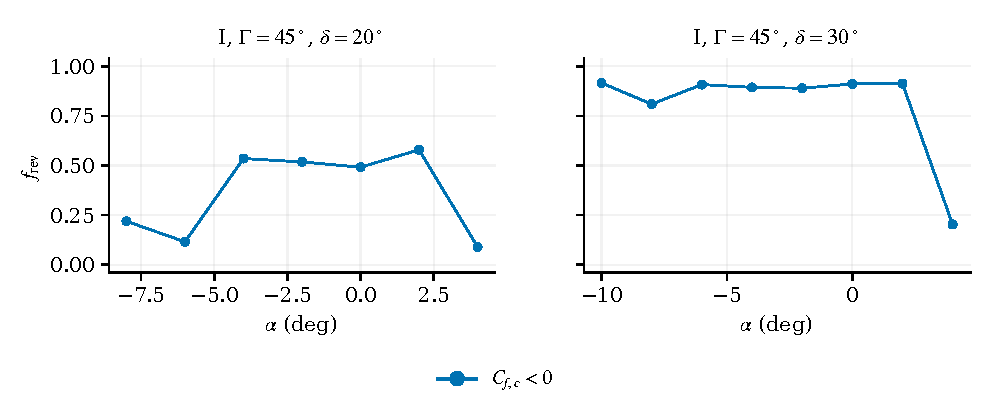
\includegraphics[width=.90\textwidth]{figures_revision_reversal_geometry.pdf}
\caption{Reverse-flow area fractions on the upper control surface for $\Gamma=45\degc$ at $\delta=20\degc$ and $\delta=30\degc$.}\label{fig:reversal_geometry}\end{figure}

Figure~\ref{fig:flow_dihedral} \DIFdelbegin \DIFdel{relates this extensive reverse flow over the control surface to the changing flow over the fixed surface. The middle row adds upper-surface $C_{f,c}$ cuts at the same span stations as the pressure sections. Between $\alpha=-2\degc$ and $\alpha=0\degc$, a band of }\DIFdelend \DIFaddbegin \DIFadd{shows }\DIFaddend increased chordwise shear \DIFdelbegin \DIFdel{develops from approximately }\DIFdelend \DIFaddbegin \DIFadd{developing from }\DIFaddend midspan toward the tip \DIFdelbegin \DIFdel{. This abrupt rise in $C_{f,c}$ is transition-like. At $\alpha=2\degc$}\DIFdelend \DIFaddbegin \DIFadd{over $\alpha=-2\to0\degc$. At $2\degc$}\DIFaddend , a narrow \DIFaddbegin \DIFadd{outboard }\DIFaddend leading-edge region \DIFdelbegin \DIFdel{of }\DIFdelend \DIFaddbegin \DIFadd{has }\DIFaddend upstream-directed \DIFdelbegin \DIFdel{chordwise shear appears over roughly the outer third of the span. At $\eta=0.8$, this short region of negative shear is followed by recovered downstream }\DIFdelend \DIFaddbegin \DIFadd{shear followed downstream by positive }\DIFaddend shear and a sharp \DIFdelbegin \DIFdel{increase in its magnitude. Together with the local pressure distribution, the pattern is }\DIFdelend \DIFaddbegin \DIFadd{rise. The accompanying pressure sections show localized suction peaks, so the combined signatures are }\DIFaddend compatible with a local \DIFdelbegin \DIFdel{separation/reattachment processand could indicate }\DIFdelend \DIFaddbegin \DIFadd{separation-and-reattachment process, possibly associated with }\DIFaddend a transition-related \DIFdelbegin \DIFdel{change in the computed boundary layer. The surface data }\DIFdelend \DIFaddbegin \DIFadd{boundary-layer change. They }\DIFaddend do not independently \DIFdelbegin \DIFdel{identify the }\DIFdelend \DIFaddbegin \DIFadd{establish the position of }\DIFaddend laminar--turbulent transition\DIFdelbegin \DIFdel{location or a complete }\DIFdelend \DIFaddbegin \DIFadd{, nor the complete topology of a }\DIFaddend three-dimensional \DIFdelbegin \DIFdel{bubble topology. On an unswept finite wing at a much lower Reynolds number, }\DIFdelend \DIFaddbegin \DIFadd{separation bubble. Measurements on a finite unswept wing by }\DIFaddend Toppings and Yarusevych~\cite{toppings2021wingtip} \DIFdelbegin \DIFdel{measured substantial spanwise variation in separation-bubble length, thickness, and reverse-flow velocity, with an open topology and eventual suppression near the tip. Spanwise variation of such features is therefore plausible on a finite wing, although those measurements do not define the present swept-wing state}\DIFdelend \DIFaddbegin \DIFadd{demonstrate that bubble-related features can vary substantially along the span, but at different Reynolds number and geometry. We use this comparison only as physical context; the present interpretation rests on the computed pressure and signed-shear fields}\DIFaddend .

\begin{figure}[htbp]\centering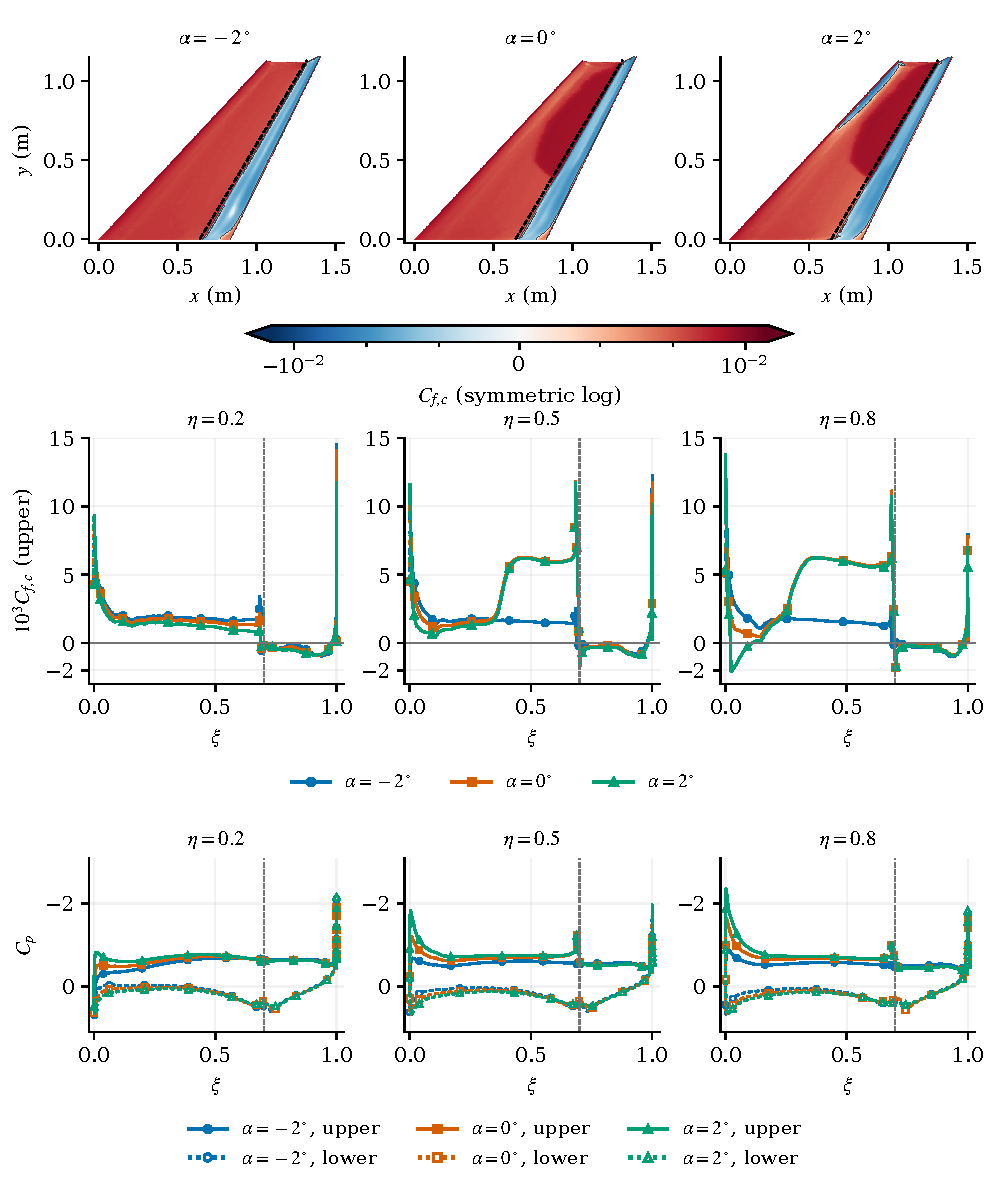
\includegraphics[width=\textwidth]{figures_revision_flow_dihedral.pdf}
\caption{$\Gamma=45\degc$, $\delta=30\degc$: upper-surface shear maps (top), upper-surface shear cuts (middle), and pressure sections (bottom) at $\alpha=-2,0,2\degc$.}\label{fig:flow_dihedral}\end{figure}

The pressure \DIFdelbegin \DIFdel{sections show the accompanying spanwise variation of loading. At $\alpha=0\degc$, the }\DIFdelend \DIFaddbegin \DIFadd{cuts show stronger }\DIFaddend leading-edge \DIFdelbegin \DIFdel{suction is weak at $\eta=0.2$, whereas distinct peaks appear at $\eta=0.5$ and $0.8$. Hinge-region suction also varies with span, with stronger peaks at the middle and outboard cuts. Stronger suction followed by pressure recoverygives }\DIFdelend \DIFaddbegin \DIFadd{and hinge-region suction at midspan and outboard stations than inboard at $\alpha=0\degc$. The larger suction is followed by recovery, giving }\DIFaddend the outboard boundary layer a different \DIFaddbegin \DIFadd{local }\DIFaddend pressure-gradient history\DIFdelbegin \DIFdel{, }\DIFdelend \DIFaddbegin \DIFadd{; this is }\DIFaddend consistent with the \DIFdelbegin \DIFdel{shear rise and }\DIFdelend \DIFaddbegin \DIFadd{spatial variation of the skin-friction increase and subsequent }\DIFaddend leading-edge \DIFdelbegin \DIFdel{reverse flow appearing there first. Spanwise variation in local inflow may contribute to the suction difference}\DIFdelend \DIFaddbegin \DIFadd{reversal}\DIFaddend . Taper reduces the \DIFdelbegin \DIFdel{local chord and , for the same section shape, the }\DIFdelend \DIFaddbegin \DIFadd{outboard chord and }\DIFaddend dimensional leading-edge radius\DIFdelbegin \DIFdel{toward the tip. The leading-edge acceleration can then occur }\DIFdelend \DIFaddbegin \DIFadd{, potentially concentrating acceleration }\DIFaddend over a shorter physical distance\DIFdelbegin \DIFdel{, increasing the spatial acceleration and pressure gradient under otherwise comparable conditions. This tendency is consistent with the stronger outboard suction, while the computed pressure distribution also reflects the coupled }\DIFdelend \DIFaddbegin \DIFadd{. Spanwise variations in effective inflow, }\DIFaddend three-dimensional flow and \DIFdelbegin \DIFdel{the spanwise change in }\DIFdelend \DIFaddbegin \DIFadd{local }\DIFaddend chord Reynolds number \DIFdelbegin \DIFdel{. Both }\DIFdelend \DIFaddbegin \DIFadd{also influence the pressure distribution, so taper alone does not establish the observed cause. Since the two }\DIFaddend dihedral configurations share this taper, \DIFdelbegin \DIFdel{so it contextualizes the spanwise variation within each model but does not explain the difference produced by }\DIFdelend \DIFaddbegin \DIFadd{it can contextualize spanwise variation *within* a planform but cannot independently explain changes due to }\DIFaddend dihedral.

\DIFdelbegin \DIFdel{Over most of the control chord, the pressure curves change little between $\alpha=-2\degc$ and $\alpha=2\degc$, consistent with the nearly unchanged reverse-flow area. The }\DIFdelend \DIFaddbegin \DIFadd{Control-chord pressure varies little over $\alpha=-2\to2\degc$ while }\DIFaddend fixed-surface \DIFdelbegin \DIFdel{shear and pressure changes therefore occur while the control remains extensively separated. The component increments in Table~\ref{tab:geometry_budget} and the $F_x/F_z$ terms in }\DIFdelend \DIFaddbegin \DIFadd{pressure and shear change substantially (}\DIFaddend Fig.~\DIFdelbegin \DIFdel{\ref{fig:dihedral}(a,b)show how this loading produces }\DIFdelend \DIFaddbegin \DIFadd{\ref{fig:flow_dihedral}). This agrees with the fixed-surface dominance of }\DIFaddend the computed moment \DIFdelbegin \DIFdel{decrease}\DIFdelend \DIFaddbegin \DIFadd{change despite extensive control reversal}\DIFaddend .
\FloatBarrier
\label{end:sec:dihedral}

\subsection{\DIFdelbegin \DIFdel{Effect of sweep direction}\DIFdelend \DIFaddbegin \DIFadd{Aft- and Forward-Swept Planforms}\DIFaddend }\label{sec:planform}
\DIFdelbegin \DIFdel{The second comparison reverses }\DIFdelend \DIFaddbegin \DIFadd{Configuration II has $-15\degc$ }\DIFaddend quarter-chord sweep \DIFdelbegin \DIFdel{from $\lambda=+30\degc$ to $\lambda=-15\degc$ while retaining the 1.6~m }\DIFdelend \DIFaddbegin \DIFadd{versus $+30\degc$ for I, with the same }\DIFaddend semispan and full-span \DIFdelbegin \DIFdel{30\%-chord control. Sweep is the principal geometric difference. Area and MAC differ by approximately 4\% and 8\%, respectively, and taper changes from 0.4 to 0.6 }\DIFdelend \DIFaddbegin \DIFadd{control. Alongside the sweep reversal, taper, chord, and area differ between these complete planforms }\DIFaddend (Table~\ref{tab:geometry})\DIFdelbegin \DIFdel{; these accompanying differences prevent attributing the response to sweep alone}\DIFdelend .

The wind-tunnel results in Fig.~\ref{fig:comparison_planform} show configuration II's local reduction in lift growth at $\delta=20\degc$ over $\alpha=0\to2\degc$: lift increases by 0.044, compared with approximately 0.092 over both $\alpha=-2\to0\degc$ and $\alpha=2\to4\degc$. Moment increases by 0.019 over $\alpha=0\to2\degc$. This feature occurs later than in configuration I, with a smaller moment rise over its interval. The primary moment departure in Table~\ref{tab:wt_geometry} exceeds both uncertainty sensitivities, although neighboring preceding fitting ranges do not uniformly exceed the primary L1 sensitivity. At $\delta=30\degc$, the reference model's broad early feature does not repeat at the same negative incidences in II.

\begin{figure}[htbp]\centering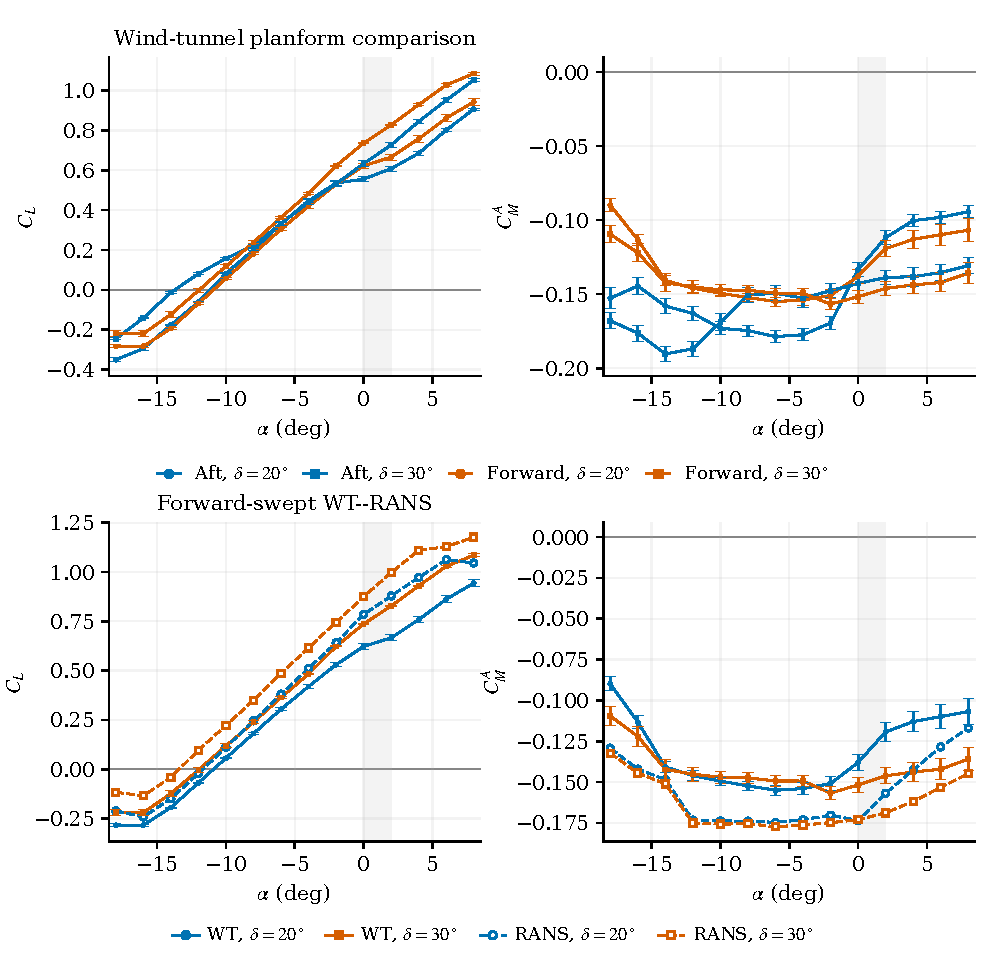
\includegraphics[width=\textwidth]{figures_revision_comparison_planform.pdf}
\caption{Wind-tunnel planform \DIFdelbeginFL \DIFdelFL{comparison (top) }\DIFdelendFL and forward-swept WT--RANS \DIFdelbeginFL \DIFdelFL{comparison (bottom)}\DIFdelendFL \DIFaddbeginFL \DIFaddFL{comparisons}\DIFaddendFL . \DIFdelbeginFL \DIFdelFL{Grey band marks }\DIFdelendFL \DIFaddbeginFL \DIFaddFL{WT bars show propagated pointwise uncertainties; grey bands mark }\DIFaddendFL the measured $\delta=20\degc$ interval.}\label{fig:comparison_planform}\end{figure}

\DIFdelbegin \DIFdel{RANS gives an $\alpha=0\to2\degc$ lift increase of 0.0935 at }\DIFdelend \DIFaddbegin \DIFadd{At }\DIFaddend $\delta=20\degc$, \DIFdelbegin \DIFdel{more than twice the measured value. Its moment increase , 0.0168, is locally close to the measured 0.019, although each moment is taken }\DIFdelend \DIFaddbegin \DIFadd{the computed lift increase over $\alpha=0\to2\degc$ is 0.0935, compared with 0.044 measured. Both WT and RANS show a positive pitching-moment increment. The numerical increment is $+0.0168$ }\DIFaddend about its own aerodynamic center\DIFdelbegin \DIFdel{. This weaker lift correspondence limits the use of its local solution to explain the measured feature}\DIFdelend \DIFaddbegin \DIFadd{, or approximately $+0.0099$ after transport to the experimental center using Eq.~\ref{eq:transport} and $\Delta C_{F,z}=0.0952$, compared with $+0.019$ measured. The spatial analysis below examines the computed load redistribution}\DIFaddend .

Figure~\ref{fig:planform_loading} \DIFdelbegin \DIFdel{shows how the two planforms redistribute loading over the same }\DIFdelend \DIFaddbegin \DIFadd{compares fixed/control, chordwise and spanwise contributions to the planform lift and moment increments over }\DIFaddend $\alpha=0\to2\degc$\DIFdelbegin \DIFdel{interval at $\Gamma=0\degc$}\DIFdelend , $\delta=20\degc$. \DIFdelbegin \DIFdel{The forward-swept fixed surface gains }\DIFdelend \DIFaddbegin \DIFadd{Configuration II has a larger fixed-surface lift gain (}\DIFaddend $+0.1014$ \DIFdelbegin \DIFdel{in lift coefficient, compared with }\DIFdelend \DIFaddbegin \DIFadd{versus }\DIFaddend $+0.0593$\DIFdelbegin \DIFdel{on I, while its control loses only }\DIFdelend \DIFaddbegin \DIFadd{) and smaller control loss (}\DIFaddend $-0.0079$ \DIFdelbegin \DIFdel{rather than }\DIFdelend \DIFaddbegin \DIFadd{versus }\DIFaddend $-0.0351$\DIFdelbegin \DIFdel{. The resulting total lift increase is larger on II, }\DIFdelend \DIFaddbegin \DIFadd{), yielding a larger total lift increment (}\DIFaddend $+0.0935$ versus $+0.0242$\DIFdelbegin \DIFdel{, but its pitching-moment increase is smaller , }\DIFdelend \DIFaddbegin \DIFadd{) but smaller moment increment (}\DIFaddend $+0.0168$ versus $+0.0339$\DIFdelbegin \DIFdel{. Each planform retains its own reference area and computed aerodynamic center. The chordwise loads locate the lift difference: the forward region gains more lift on II, }\DIFdelend \DIFaddbegin \DIFadd{). Along the chord, II gains lift in }\DIFaddend the intermediate region \DIFdelbegin \DIFdel{gains }\DIFdelend \DIFaddbegin \DIFadd{(}\DIFaddend $+0.0063$\DIFdelbegin \DIFdel{instead of losing }\DIFdelend \DIFaddbegin \DIFadd{), where I loses it (}\DIFaddend $-0.0097$\DIFdelbegin \DIFdel{, and the aft loss is reduced from $-0.0332$ on I to }\DIFdelend \DIFaddbegin \DIFadd{), and has much smaller aft losses (}\DIFaddend $-0.0065$ \DIFdelbegin \DIFdel{on II. The smaller }\DIFdelend \DIFaddbegin \DIFadd{versus $-0.0332$). The forward region gains lift on both models, but the differing }\DIFaddend intermediate and aft \DIFdelbegin \DIFdel{moment increments on II, with similar forward-region contributions, accompany this redistribution. }\DIFdelend \DIFaddbegin \DIFadd{increments distinguish their redistribution. These are per-configuration normalized coefficient increments about their respective aerodynamic centers, so the comparison is of the complete planform responses rather than a force difference at one common moment pole.
}\DIFaddend 

\begin{figure}[htbp]\centering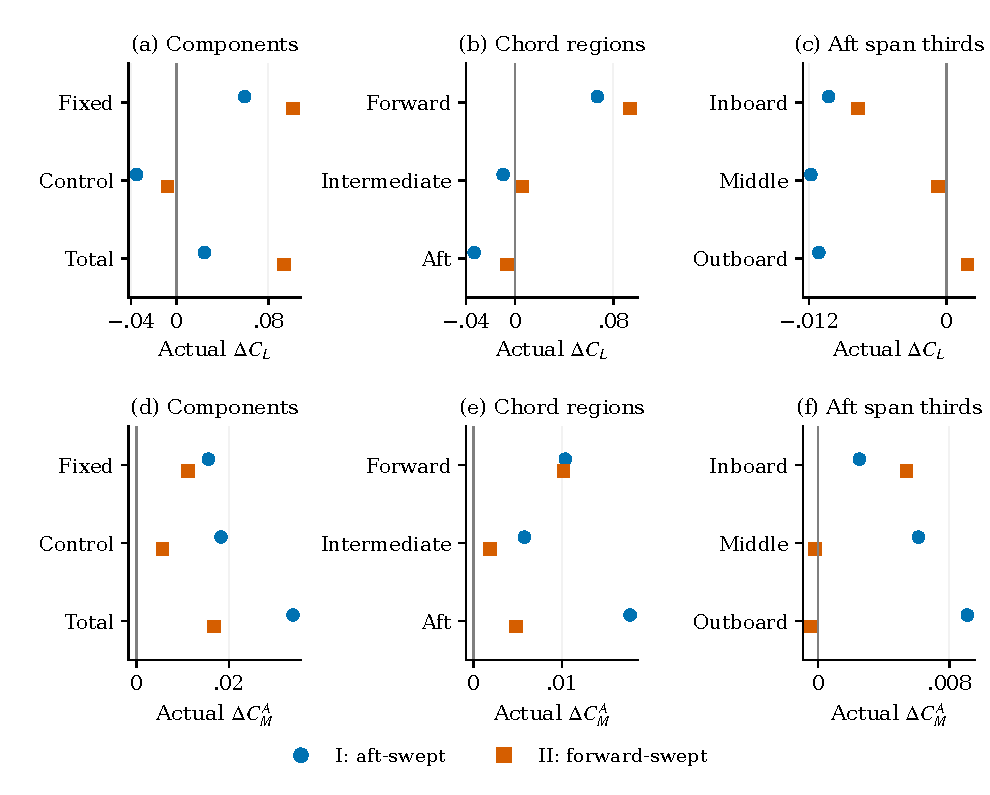
\includegraphics[width=\textwidth]{figures_revision_planform_loading.pdf}
\caption{Planform comparison over $\alpha=0\to2\degc$, $\delta=20\degc$: lift increments (top) and aerodynamic-center moment increments (bottom), with matching decompositions.}\label{fig:planform_loading}\end{figure}

\begin{figure}[!tp]\centering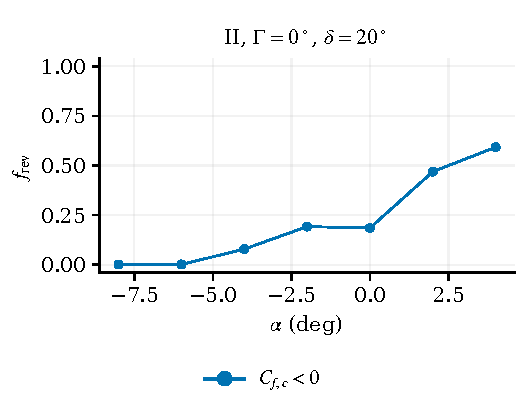
\includegraphics[width=.50\textwidth]{figures_revision_reversal_planform.pdf}
\caption{Forward-swept upper control surface reverse-flow area fraction at $\delta=20\degc$; the open diamond marks $\alpha=0\degc$, the start of the interval in the loading analysis.}\label{fig:reversal_planform}\end{figure}

The \DIFdelbegin \DIFdel{pitching response depends additionally on where the aft force changes occur relative to the moment axis}\DIFdelend \DIFaddbegin \DIFadd{aft loading also shifts spanwise}\DIFaddend . On I, comparable aft lift losses occur across the span, \DIFdelbegin \DIFdel{yet }\DIFdelend \DIFaddbegin \DIFadd{but }\DIFaddend the positive moment \DIFdelbegin \DIFdel{increments increase toward the tip}\DIFdelend \DIFaddbegin \DIFadd{contribution increases outboard as the downstream arm grows with aft sweep}\DIFaddend . On II, aft \DIFdelbegin \DIFdel{lift }\DIFdelend loss and positive moment change are concentrated inboard, while the outboard aft region gains lift\DIFdelbegin \DIFdel{. The aft regions lie downstream of the respective numerical aerodynamic centers, but the streamwise arm $x-x_A$ increases outboard on I and decreases on II. Consequently, for an equal loss of upward force, the }\DIFdelend \DIFaddbegin \DIFadd{; the downstream arm instead decreases toward the tip. The factor }\DIFaddend $-(x-x_A)dF_z$ \DIFdelbegin \DIFdel{term in Eq. ~\ref{eq:moment} gives a larger positive moment contribution outboard on I. These different spanwise }\DIFdelend \DIFaddbegin \DIFadd{therefore gives a different spanwise weighting of the }\DIFaddend force changes and \DIFdelbegin \DIFdel{moment arms explain why the }\DIFdelend \DIFaddbegin \DIFadd{helps explain why II's }\DIFaddend larger total lift increase \DIFdelbegin \DIFdel{on II }\DIFdelend does not produce a larger \DIFdelbegin \DIFdel{pitching-moment increase. }\DIFdelend \DIFaddbegin \DIFadd{moment increment. The contributions also depend on the actual local force distribution, not on a moment-arm factor applied to a uniform span load. Earlier forward-swept-wing observations by }\DIFaddend McCormack and Cook~\cite{mccormack1949sweptforward} \DIFdelbegin \DIFdel{documented a related role of inboard chordwise load location on a 45$\degc$ forward-swept }\DIFdelend \DIFaddbegin \DIFadd{link inboard pressure redistribution to pitching moment in a }\DIFaddend wing without controls\DIFdelbegin \DIFdel{. In its moderate-lift range, failed aft pressure recovery over the inboard sections shifted their centers of pressure rearward with little change in section lift , spread outboard with incidence, and changed the wing pitching moment before the lift-curve slope decreased. That stall study differs in section, Reynolds number, and control configuration, but it similarly shows that the chordwise and spanwise location of inboard load changes can govern the forward-swept pitching response.
}\DIFdelend \DIFaddbegin \DIFadd{; that prior result is context rather than a directly matching loading mechanism.
}\DIFaddend 

\DIFdelbegin \DIFdel{Actual lift growth can still fall short of its preceding trend. The }\DIFdelend \DIFaddbegin \DIFadd{Despite its larger actual lift increment, II also falls below the preceding trend: its }\DIFaddend fixed/control \DIFdelbegin \DIFdel{lift }\DIFdelend departures are $-0.0263/-0.0104$\DIFdelbegin \DIFdel{on II, compared with }\DIFdelend \DIFaddbegin \DIFadd{, against }\DIFaddend $-0.0692/-0.0414$ on I\DIFdelbegin \DIFdel{; even II's positive intermediate-region increment represents reduced growth relative to that trend}\DIFdelend . Moment departures about the \DIFdelbegin \DIFdel{computed }\DIFdelend \DIFaddbegin \DIFadd{respective }\DIFaddend aerodynamic centers reinforce \DIFdelbegin \DIFdel{each other, with the control contribution larger on I and the two contributions similar on II . At II's }\DIFdelend \DIFaddbegin \DIFadd{in both cases, but the II contributions partly cancel about its }\DIFaddend original numerical origin \DIFdelbegin \DIFdel{, however, the fixed/control departures are }\DIFdelend \DIFaddbegin \DIFadd{(}\DIFaddend $-0.0023/+0.0035$\DIFdelbegin \DIFdel{and partly cancel. The following shear and pressure distributions locate the control-surface flow changes accompanying these integrated differences}\DIFdelend \DIFaddbegin \DIFadd{)}\DIFaddend .

\DIFdelbegin \DIFdel{Figure~\ref{fig:reversal_planform} places the increase in II's reverse-flow area fraction beside its loading analysis. The }\DIFdelend \DIFaddbegin \DIFadd{On II, the }\DIFaddend upper-control \DIFdelbegin \DIFdel{fraction grows }\DIFdelend \DIFaddbegin \DIFadd{reversed-shear fraction rises }\DIFaddend from about 19\% to 47\% and 59\% at $\alpha=0,2,4\degc$ \DIFaddbegin \DIFadd{(Fig.~\ref{fig:reversal_planform})}\DIFaddend . The surface maps in Fig.~\ref{fig:flow_planform} \DIFdelbegin \DIFdel{show where this change occurs: at $\alpha=0\degc$, reverse flow near the trailing edge is concentrated around midspan ; with increasing incidence, it extends upstream }\DIFdelend \DIFaddbegin \DIFadd{locate the growth chiefly around midspan and then increasingly toward the root, with upstream spreading }\DIFaddend along the control chord\DIFdelbegin \DIFdel{and toward the root. The pressure sections across $\alpha=0\to2\degc$ show a weakened upper-side hinge-suction peak inboard }\DIFdelend \DIFaddbegin \DIFadd{. Over the same 0--2-degree interval, the pressure cuts show weakened inboard hinge suction }\DIFaddend and comparatively little change at the outboard \DIFdelbegin \DIFdel{cut}\DIFdelend \DIFaddbegin \DIFadd{section}\DIFaddend , consistent with the \DIFaddbegin \DIFadd{inboard }\DIFaddend concentration of aft lift loss\DIFdelbegin \DIFdel{inboard}\DIFdelend \DIFaddbegin \DIFadd{. These observations connect the chordwise and spanwise load integrals to the evolving near-wall signature without assuming that its area fraction alone determines the force}\DIFaddend .

\begin{figure}[!tp]\centering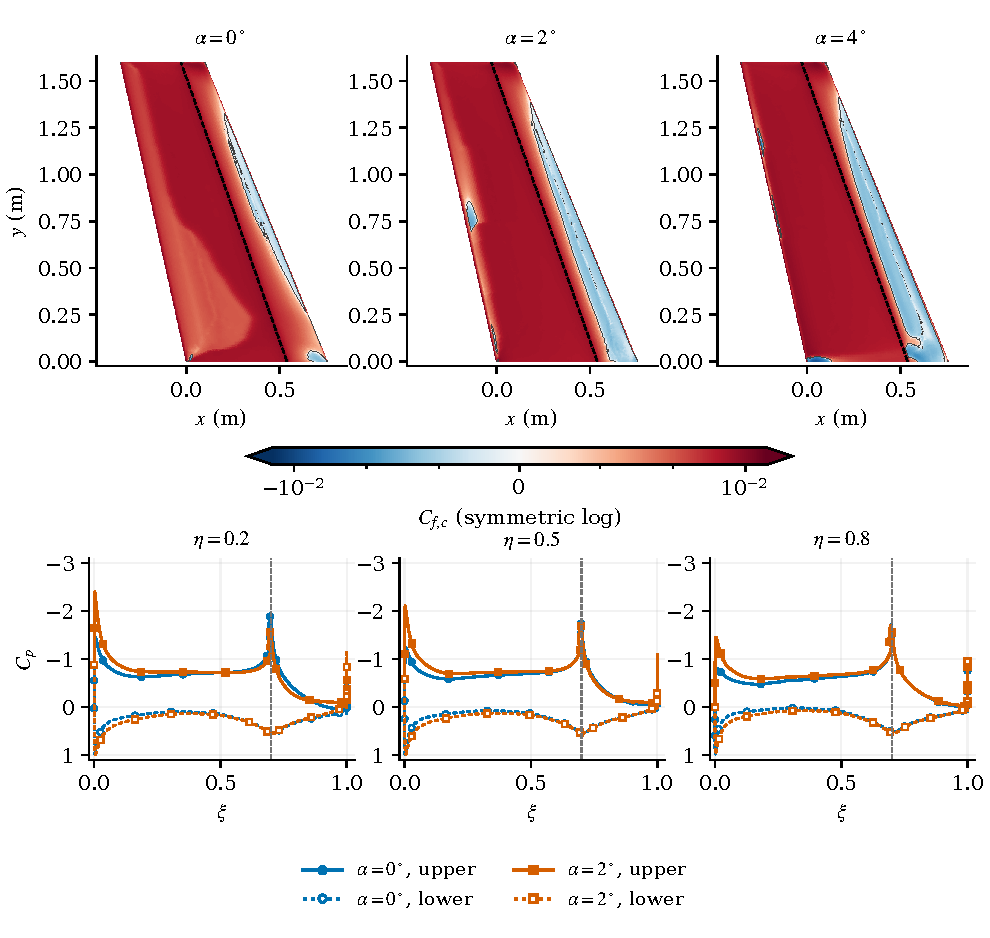
\includegraphics[width=.90\textwidth]{figures_revision_flow_planform.pdf}
\caption{Forward-swept planform, $\delta=20\degc$: upper-surface chordwise shear (top) and pressure sections across $\alpha=0\to2\degc$ (bottom).}\label{fig:flow_planform}\end{figure}

At \DIFdelbegin \DIFdel{$\alpha=2\degc$, II 's reverse-flow area fraction is close to I 's }\DIFdelend \DIFaddbegin \DIFadd{$2\degc$, II and I have similar reversed-shear fractions (about 47\% and }\DIFaddend 49\%\DIFdelbegin \DIFdel{, despite its much smaller control lift loss across $\alpha=0\to2\degc$. The differing }\DIFdelend \DIFaddbegin \DIFadd{) but markedly different control lift losses. Their }\DIFaddend pressure distributions and load locations\DIFdelbegin \DIFdel{explain why comparable reverse-flow areas can accompany different lift and moment changes. Together, the two planform comparisons show how fixed-surface growth, control loss, and their chordwise/spanwise locations combine in the integrated response}\DIFdelend \DIFaddbegin \DIFadd{—not reversed-shear area alone—account for the different integrated responses}\DIFaddend .
\label{end:sec:planform}
\FloatBarrier
\label{end:sec:geometry_effects}
\section{Conclusions}\label{sec:conclusions}
The wind-tunnel measurements show that \DIFdelbegin \DIFdel{reductions in }\DIFdelend pre-stall \DIFdelbegin \DIFdel{lift growth and changes in pitching moment do not necessarily occur over the same incidence interval or at the same }\DIFdelend \DIFaddbegin \DIFadd{lift-growth reductions and pitching-moment changes need not coincide in incidence or }\DIFaddend control deflection. \DIFdelbegin \DIFdel{Resolving the computed forces into fixed- and control-surface contributions, then examining their spatial distribution, identifies how different combinations of loading changes produce the numerical lift and pitching responses.
}%DIFDELCMD < 

%DIFDELCMD < %%%
\DIFdel{The reference computation shows that continued total lift growth can conceal reduced growth on both }\DIFdelend \DIFaddbegin \DIFadd{Decomposing the computed loads identifies the different contributions of }\DIFaddend the fixed surface and the full-span control. For \DIFdelbegin \DIFdel{configuration I at zero dihedral and }\DIFdelend \DIFaddbegin \DIFadd{the aft-swept, zero-dihedral model at }\DIFaddend $\delta=20\degc$, \DIFdelbegin \DIFdel{fixed lift gain exceeds actual control lift loss, yet }\DIFdelend \DIFaddbegin \DIFadd{total lift still increases over $\alpha=0\to2\degc$, but }\DIFaddend the fixed surface accounts for \DIFdelbegin \DIFdel{approximately }\DIFdelend \DIFaddbegin \DIFadd{about }\DIFaddend 63\% of the \DIFdelbegin \DIFdel{total departure below the preceding trend. The control contributes more strongly to the positive }\DIFdelend \DIFaddbegin \DIFadd{shortfall relative to the preceding lift-growth trend; the control produces the larger }\DIFaddend pitching-moment departure about the numerical aerodynamic center.

\DIFdelbegin \DIFdel{Pressure sections and regional integrations explain why stronger }\DIFdelend \DIFaddbegin \DIFadd{Stronger }\DIFaddend leading-edge suction \DIFdelbegin \DIFdel{is consistent with reduced fixed-surface growth : the forward-region gain falls below its preceding trend, while the intermediate region actually loses lift. Similar }\DIFdelend \DIFaddbegin \DIFadd{accompanies reduced growth over the forward chord and actual lift loss over the intermediate chord. Comparable }\DIFaddend aft lift losses \DIFdelbegin \DIFdel{produce }\DIFdelend \DIFaddbegin \DIFadd{yield progressively }\DIFaddend larger positive moment increments \DIFdelbegin \DIFdel{outboard as their downstream moment arms grow. The upper-control shear pattern shifts from reverse flow adjacent to the hinge to reverse flow near the trailing edge across the computed interval. Its subsequent upstream extension coexists with renewed total lift growth. Consequently, the extent of reverse flow complements the pressure and load evidence but does not determine the integrated response by itself.
}%DIFDELCMD < 

%DIFDELCMD < %%%
\DIFdel{The measurements establish distinct lift and momentresponses across deflection and geometry. RANS reproduces the principal reference trends with a displaced lift interval and substantial coefficient-level bias, while correspondence is weaker for the dihedral and forward-swept cases. The detailed loading findings therefore characterize the computed flow fields and loads}\DIFdelend \DIFaddbegin \DIFadd{toward the tip because the aft-swept moment arms increase outboard. Changes in control-surface reverse flow accompany these load changes, but reversal area alone cannot predict integrated lift or moment}\DIFaddend .

\DIFdelbegin \DIFdel{For matched }\DIFdelend \DIFaddbegin \DIFadd{With $45\degc$ }\DIFaddend dihedral, adjacent lift increments reverse their ordering \DIFdelbegin \DIFdel{between the two orientations. The common-axis moment comparison also changes from reinforcement to compensation between the contributions from $F_x$ and $F_z$ across incidence intervals. Both the force magnitudes and their moment arms enter this incidence-dependent response. }%DIFDELCMD < 

%DIFDELCMD < %%%
\DIFdelend \DIFaddbegin \DIFadd{relative to the zero-dihedral model, while the axial- and normal-force moment contributions alternately reinforce and partly compensate about a common reference axis. }\DIFaddend The forward-swept planform \DIFdelbegin \DIFdel{gives stronger }\DIFdelend \DIFaddbegin \DIFadd{exhibits greater }\DIFaddend fixed-surface lift growth, \DIFdelbegin \DIFdel{much weaker control loss, positive intermediate-chord growth }\DIFdelend \DIFaddbegin \DIFadd{weaker control losses }\DIFaddend and an inboard-concentrated \DIFdelbegin \DIFdel{aft lift loss over the matched $\alpha=0\to2\degc$ interval. Consequently, its aft moment increments lack the reference model's increase in positive moment contribution toward the tip about the corresponding aerodynamic centers. This connects the different pitching responses to the chordwise and spanwise organization of the computed loading}\DIFdelend \DIFaddbegin \DIFadd{aft-loading change. These comparisons show that the magnitude and spatial distribution of load changes both shape the pitching-moment response}\DIFaddend .

\DIFdelbegin \DIFdel{Future computations on the finer levels of the established mesh hierarchy are planned to assess the resolution sensitivity of the }\DIFdelend \DIFaddbegin \DIFadd{Finer-grid studies can further assess the }\DIFaddend pre-stall \DIFdelbegin \DIFdel{load redistribution, with particular attention to pitching moment and the fixed- and control-surface contributions. The present joint analysis identifies how continued lift growth can coexist with different component lift deficits and pitching-moment contributions}\DIFdelend \DIFaddbegin \DIFadd{component moments. The results show why continuing total lift growth does not, by itself, reveal where force changes governing pitching moment occur}\DIFaddend .
\appendix
\label{end:sec:conclusions}
\section{Sensitivity Checks}\label{app:sensitivity}
\DIFdelbegin \DIFdel{This appendix checks three choices made in the analysis. The departures depend on the preceding incidence samples that define each fitted trend (Sec.~\ref{sec:analysis}). Their regional values also depend on how the surface is divided (Sec.~\ref{sec:pressure}). The reverse-flow area fraction depends on the sign criterion $C_{f,c}<0$ (Sec.~\ref{sec:analysis}). The checks follow this order, from the fitted trend to the regions and then to the near-wall flow. The appendix ends with one feature of the stored solutions that is not interpreted}\DIFdelend \DIFaddbegin \DIFadd{The following checks assess sensitivity to preceding-incidence fits, integration partitions and the reverse-shear threshold}\DIFaddend .

\DIFdelbegin \DIFdel{The first check concerns the preceding trend. Table~\ref{tab:sensitivity} lists the reference $\delta=20\degc$, $\alpha=0\to2\degc$ lift allocation for }\DIFdelend \DIFaddbegin \DIFadd{Across }\DIFaddend three preceding-incidence fitting ranges\DIFdelbegin \DIFdel{. The }\DIFdelend \DIFaddbegin \DIFadd{, the reference }\DIFaddend fixed-surface \DIFdelbegin \DIFdel{fraction }\DIFdelend \DIFaddbegin \DIFadd{share of the lift-growth shortfall }\DIFaddend remains 62.4--62.6\%, while the total \DIFdelbegin \DIFdel{lift }\DIFdelend departure varies from \DIFdelbegin \DIFdel{approximately }\DIFdelend $-0.105$ to $-0.137$ \DIFdelbegin \DIFdel{. The allocation therefore varies much less than the departure amplitude. These rows quantify robustness to the empirical preceding trend; they are neither a confidence interval nor a grid-convergence estimate}\DIFdelend \DIFaddbegin \DIFadd{(Table~\ref{tab:sensitivity}). These checks do not represent confidence intervals or grid-error bounds}\DIFaddend .

\begin{table}[htbp]\centering\small
\caption{Reference loading departures over $\alpha=0\to2\degc$, $\delta=20\degc$: sensitivity to the preceding incidence samples; moments are about the computed aerodynamic center.}\label{tab:sensitivity}
\begin{tabular}{lrrr}\toprule
Preceding $\alpha$ (deg) & Total $D_L$ & Fixed fraction (\%) & Total $D_M$ \\\midrule
\tablerows{tables_revision_sensitivity_rows}
\bottomrule\end{tabular}\end{table}

\DIFdelbegin \DIFdel{With the complete departures checked, the same question applies to their regional division. }\DIFdelend Figure~\ref{fig:partition_check} \DIFdelbegin \DIFdel{shows the two partitions used to check the regional interpretation. The first divides the semispan into thirds and the chord at the hinge; the second uses spanwise quarters and adds a chord boundary at $\xi=0.4$}\DIFdelend \DIFaddbegin \DIFadd{compares spanwise-third and spanwise-quarter partitions, with alternative chord subdivisions}\DIFaddend .

\begin{figure}[htbp]\centering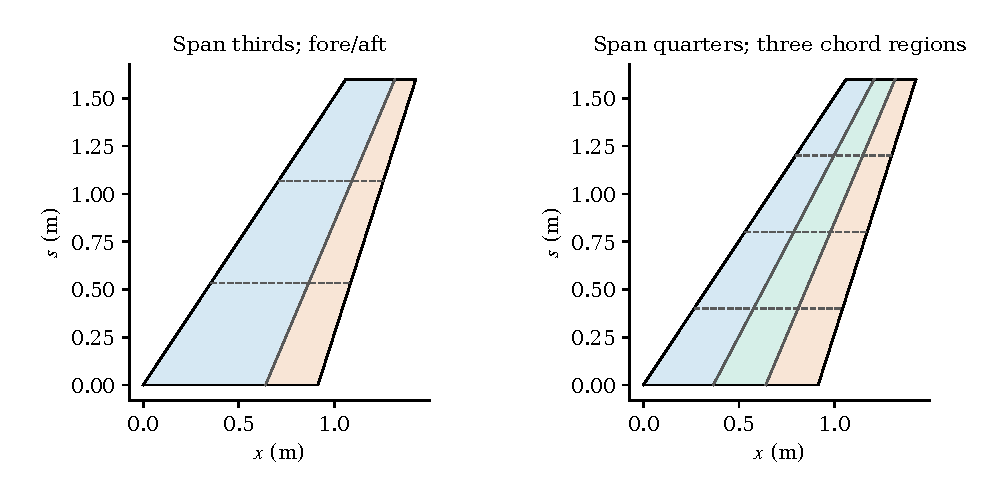
\includegraphics[width=.80\textwidth]{figures_revision_partition_check.pdf}
\caption{Alternative integration partitions: spanwise thirds with fore/aft regions (left), and quarters with forward/intermediate/aft regions (right).}\label{fig:partition_check}\end{figure}
\FloatBarrier

Moving the spanwise boundary from one third to one quarter changes the inboard aft departure from approximately $-0.0127$ to $-0.00939$, while complete fore/aft sums remain unchanged. Finer chord subdivisions preserve the two negative fixed-chord departures. These checks support the complete loading interpretation while showing that individual regional contributions depend on the partition.

The main text compares \DIFdelbegin \DIFdel{the regional loads with the }\DIFdelend \DIFaddbegin \DIFadd{chordwise and spanwise load changes with the extent of upstream-directed }\DIFaddend near-wall \DIFdelbegin \DIFdel{flow }\DIFdelend \DIFaddbegin \DIFadd{shear }\DIFaddend on the control\DIFdelbegin \DIFdel{, measured by the reverse-flow area fraction}\DIFdelend . Replacing the zero threshold with small negative values, $C_{f,c}<-10^{-6}$ and $C_{f,c}<-10^{-5}$, leaves the reference result nearly unchanged. With the larger threshold, the $\delta=20\degc$ fraction grows from 0.145 to 0.480 across $\alpha=0\to2\degc$, compared with 0.146 to 0.485 in Fig.~\ref{fig:reversal}. These threshold checks and the fractions over other geometric partitions are retained in the reproducibility record; the main figures use $C_{f,c}<0$.

\label{anchor:saved_state}The same measure shows a feature of the stored $\Gamma=45\degc$ solutions that is not interpreted. The upper control surface reverse-flow area fractions decrease between $\alpha=2\degc$ and $\alpha=4\degc$, from about 0.58 to 0.09 at $\delta=20\degc$ and from 0.91 to 0.20 at $\delta=30\degc$. Their physical origin remains unresolved, so we do not interpret them as a transition or reattachment sequence.
\label{end:app:sensitivity}
\FloatBarrier
\section*{Acknowledgments}\label{anchor:acknowledgments}
This project has received funding from the Clean Sky 2 Joint Undertaking (JU) under grant agreement No 101008257. The JU receives support from the European Union's Horizon 2020 research and innovation programme and the Clean Sky 2 JU members other than the Union.

The authors used generative artificial intelligence tools (Claude, Anthropic, and Codex, OpenAI) to assist in writing the scripts that post-processed the existing wind-tunnel and numerical data and produced the figures, and to assist in drafting and editing the text and improving its grammar and correctness. Grammarly was used to check the syntax. No data were generated by these tools. The authors reviewed and verified all scripts, figures, and text, and take full responsibility for the content of this paper.
\label{anchor:references}\bibliography{References}
\label{end:references}
\end{document}
